% =====================================================================
% RESOLUCAO COMPLETA — Listas DCA 1, 2 e 3
% 18 Problemas com Demonstracoes Integrais
% Formato ABNT NBR 14724 — GeoMaker+IA
% Cada "mostre que" e EFETIVAMENTE demonstrado
% =====================================================================
\documentclass[12pt,a4paper,oneside]{article}
\usepackage[utf8]{inputenc}
\usepackage[T1]{fontenc}
\usepackage{lmodern}
\usepackage[brazil]{babel}
\usepackage{geometry}
\geometry{margin=3cm,top=3cm,bottom=2cm}
\usepackage{indentfirst}
\setlength{\parindent}{1.25cm}
\usepackage{setspace}
\onehalfspacing
\usepackage{microtype}
\usepackage{amsmath,amssymb,amsthm}
\usepackage{booktabs,array,longtable,multirow,tabularx}
\usepackage{graphicx}
\usepackage{hyperref}
\usepackage{enumitem}
\usepackage{xcolor}
\usepackage{colortbl}
\usepackage{float}
\usepackage{caption}
\usepackage{fancyhdr}
\hypersetup{colorlinks=true,linkcolor=blue,citecolor=blue,urlcolor=blue}
\definecolor{greenbg}{HTML}{d4edda}

\newtheorem{lemma}{Lema}
\newtheorem{proofstep}{Passo}

\pagestyle{fancy}
\fancyhf{}
\fancyhead[R]{\small GeoMaker+IA — CNM 9.76.35.5698}
\fancyfoot[C]{\thepage}

\begin{document}

\begin{center}
{\LARGE \textbf{Resolucao Completa — Listas DCA 1, 2 e 3}}\\[12pt]
{\large 18 Problemas com Demonstracoes Integrais}\\[6pt]
{\large Dinamica Classica Avancada — Macedo (2026)}\\[6pt]
{\large GeoMaker+IA — Museu Escolar Itinerante (CNM 9.76.35.5698)}\\[6pt]
{\large 27 de Maio de 2026}
\end{center}
\thispagestyle{empty}
\newpage

% =====================================================================
\section{Lista 1 — Questao 1: Identidades Simpleticas [2,0 pts]}

\textbf{Enunciado:} Seja $(M,\Omega)$ uma variedade simpletica. Para cada
funcao suave $F$, defina o campo Hamiltoniano $X_F$ por $i_{X_F}\Omega=-dF$
e o parentese de Poisson por $\{F,G\}=X_G(F)$. Sem introduzir coordenadas
locais, prove usando apenas calculo exterior, produto interior e derivada
de Lie:

(a) $[X_F,X_G] = -X_{\{F,G\}}$

(b) $\mathcal{L}_{X_F}G = \{G,F\}$ e $\mathcal{L}_{X_F}\Omega = 0$

(c) $\frac{dH}{dt} = \mathcal{L}_{X_H}H = 0$, com interpretacao geometrica

(d) Deduza a identidade de Jacobi dos parenteses de Poisson da identidade
de Jacobi do colchete de Lie.

% -------------------------------------------------------------------
\subsection*{Pre-requisitos}

Antes de iniciar as demonstracoes, recordamos tres identidades do calculo
exterior que serao usadas:

\begin{enumerate}[label=\textbf{(I\arabic*)}, leftmargin=*]
  \item \textbf{Formula Magica de Cartan:} Para qualquer campo vetorial $X$
        e forma diferencial $\alpha$:
        $$\mathcal{L}_X\alpha = i_X(d\alpha) + d(i_X\alpha)$$
  \item \textbf{Lema de Poincare:} $d^2 = 0$, ou seja, $d(d\alpha)=0$ para
        qualquer forma $\alpha$.
  \item \textbf{Identidade fundamental do colchete de Lie:}
        $$i_{[X,Y]} = \mathcal{L}_X \circ i_Y - i_Y \circ \mathcal{L}_X$$
        onde $[X,Y]$ e o colchete de Lie e $\circ$ denota composicao.
\end{enumerate}

\subsection*{Demonstracao de (a): $[X_F,X_G] = -X_{\{F,G\}}$}

\textbf{Passo 1.} Aplicamos a identidade (I3) com $X=X_F$ e $Y=X_G$,
avaliando ambos os lados sobre a 2-forma $\Omega$:

\begin{equation}\label{eq:a1}
i_{[X_F,X_G]}\Omega = \mathcal{L}_{X_F}\big(i_{X_G}\Omega\big) -
i_{X_G}\big(\mathcal{L}_{X_F}\Omega\big)
\end{equation}

\textbf{Passo 2.} Calculamos $\mathcal{L}_{X_F}\Omega$ usando a Formula de
Cartan (I1):

\begin{align}
\mathcal{L}_{X_F}\Omega &= i_{X_F}(d\Omega) + d(i_{X_F}\Omega) \notag\\
&= i_{X_F}(0) + d(-dF) \notag\\
&= 0 + (-d^2F) \notag\\
&= 0 \label{eq:a2}
\end{align}

Justificativa de cada linha: (i) $\Omega$ e uma forma simpletica, portanto
e fechada por definicao: $d\Omega = 0$. (ii) Pela definicao de $X_F$,
$i_{X_F}\Omega = -dF$. (iii) $d(-dF) = -d(dF) = -d^2F$. (iv) Pelo Lema de
Poincare (I2), $d^2F = 0$.

O resultado $\mathcal{L}_{X_F}\Omega = 0$ significa que o fluxo Hamiltoniano
\textbf{preserva a forma simpletica} — e o Teorema de Liouville em sua forma
geometrica.

\textbf{Passo 3.} Substituindo (\ref{eq:a2}) em (\ref{eq:a1}), o segundo
termo se anula:

$$i_{[X_F,X_G]}\Omega = \mathcal{L}_{X_F}\big(i_{X_G}\Omega\big) - 0$$

Usando a definicao de $X_G$ ($i_{X_G}\Omega = -dG$):

\begin{equation}\label{eq:a3}
i_{[X_F,X_G]}\Omega = \mathcal{L}_{X_F}(-dG) = -\mathcal{L}_{X_F}(dG)
\end{equation}

\textbf{Passo 4.} Uma propriedade fundamental do calculo exterior e que a
derivada de Lie comuta com a derivada exterior quando aplicada a funcoes
(0-formas). Demonstramos esta propriedade:

$$\mathcal{L}_X(df) = i_X\big(d(df)\big) + d\big(i_X(df)\big)$$

O primeiro termo e $i_X(d^2f) = i_X(0) = 0$ (Poincare). O segundo termo e
$d(X(f))$ pois $i_X(df) = df(X) = X(f)$. Portanto:

$$\mathcal{L}_X(df) = d(X(f)) = d(\mathcal{L}_X f)$$

Aplicando esta propriedade ao lado direito de (\ref{eq:a3}):

\begin{align}
i_{[X_F,X_G]}\Omega &= -d\big(\mathcal{L}_{X_F} G\big) \notag\\
&= -d\big(X_F(G)\big) \label{eq:a4}
\end{align}

onde usamos que $\mathcal{L}_{X_F}G = X_F(G)$ para uma funcao $G$.

\textbf{Passo 5.} Pela definicao do parentese de Poisson:
$\{F,G\} = X_G(F)$. Trocando $F$ e $G$: $\{G,F\} = X_F(G)$.

Substituindo em (\ref{eq:a4}):

\begin{equation}\label{eq:a5}
i_{[X_F,X_G]}\Omega = -d\big(\{G,F\}\big)
\end{equation}

\textbf{Passo 6.} Por definicao, o campo Hamiltoniano de uma funcao $H$
satisfaz $i_{X_H}\Omega = -dH$. Aplicando a $H = \{G,F\}$:

\begin{equation}\label{eq:a6}
i_{X_{\{G,F\}}}\Omega = -d\big(\{G,F\}\big)
\end{equation}

\textbf{Passo 7.} Comparando (\ref{eq:a5}) e (\ref{eq:a6}):

$$i_{[X_F,X_G]}\Omega = i_{X_{\{G,F\}}}\Omega$$

\textbf{Passo 8.} A forma simpletica $\Omega$ e nao-degenerada. Isto
significa que a aplicacao $X \mapsto i_X\Omega$ do fibrado tangente no
fibrado cotangente e um isomorfismo. Em particular, e injetiva:

$$i_X\Omega = i_Y\Omega \;\Longrightarrow\; X = Y$$

Aplicando este fato com $X = [X_F,X_G]$ e $Y = X_{\{G,F\}}$:

$$[X_F,X_G] = X_{\{G,F\}}$$

\textbf{Passo 9.} O parentese de Poisson e antissimetrico. Demonstramos:

\begin{align*}
\{G,F\} &= X_F(G) = dG(X_F) \\
&= dG\big(\Omega^{-1}(-dF, \cdot)\big) \quad\text{(pois } X_F = \Omega^{-1}(-dF,\cdot))\\
&= -\Omega^{-1}(dF, dG) \\
&= -\{F,G\}
\end{align*}

Portanto, $\{G,F\} = -\{F,G\}$. Consequentemente:

$$[X_F,X_G] = X_{-\{F,G\}} = -X_{\{F,G\}}$$

que e exatamente a identidade que queriamos demonstrar. $\square$

\subsection*{Demonstracao de (b): $\mathcal{L}_{X_F}G = \{G,F\}$ e
$\mathcal{L}_{X_F}\Omega = 0$}

\textbf{Primeira identidade.} Para uma funcao suave $G$ (0-forma), a
derivada de Lie ao longo de $X_F$ e simplesmente a derivada direcional:

$$\mathcal{L}_{X_F}G = X_F(G)$$

Pela definicao do parentese de Poisson com argumentos trocados,
$\{G,F\} = X_F(G)$. Logo:

$$\mathcal{L}_{X_F}G = \{G,F\}$$

\textbf{Segunda identidade.} Ja foi demonstrada no Passo 2 da parte (a),
onde obtivemos $\mathcal{L}_{X_F}\Omega = 0$ usando a Formula de Cartan,
$d\Omega = 0$, $i_{X_F}\Omega = -dF$, e $d^2 = 0$. $\square$

\subsection*{Demonstracao de (c): $\mathcal{L}_{X_H}H = 0$}

A derivada de Lie de $H$ ao longo de $X_H$ e:

$$\mathcal{L}_{X_H}H = X_H(H) = dH(X_H)$$

Mas $dH = -i_{X_H}\Omega$ (da definicao de $X_H$). Portanto:

\begin{align*}
\mathcal{L}_{X_H}H &= (-i_{X_H}\Omega)(X_H) \\
&= -i_{X_H}\Omega(X_H) \\
&= -\Omega(X_H, X_H)
\end{align*}

Como $\Omega$ e uma 2-forma antissimetrica, $\Omega(X_H, X_H) = 0$ para
qualquer campo $X_H$. Equivalentemente, usando $\Omega^{-1}$:

$$\mathcal{L}_{X_H}H = \Omega^{-1}(dH, dH) = 0$$

pela antissimetria de $\Omega^{-1}$. $\square$

\textbf{Interpretacao geometrica:} O Hamiltoniano $H$ e \textbf{conservado
ao longo das curvas integrais} do seu proprio campo $X_H$. As trajetorias
do sistema permanecem confinadas as superficies de nivel $H = \text{constante}$.
Em termos fisicos, e a \textbf{lei de conservacao da energia}: a energia
total de um sistema Hamiltoniano isolado nao varia com o tempo.

\subsection*{Demonstracao de (d): Jacobi de Poisson $\to$ Jacobi de Lie}

Queremos provar que, para quaisquer funcoes suaves $F, G, H$:

$$\{F,\{G,H\}\} + \{G,\{H,F\}\} + \{H,\{F,G\}\} = 0$$

\textbf{Passo 1.} Usamos a identidade operatoria entre Lie derivatives:

\begin{equation}\label{eq:d1}
[\mathcal{L}_X, \mathcal{L}_Y] = \mathcal{L}_{[X,Y]}
\end{equation}

que e uma consequencia direta da definicao de colchete de Lie. O lado
esquerdo e o comutador de operadores: $[\mathcal{L}_X,\mathcal{L}_Y] =
\mathcal{L}_X \circ \mathcal{L}_Y - \mathcal{L}_Y \circ \mathcal{L}_X$.

\textbf{Passo 2.} Aplicamos (\ref{eq:d1}) a uma funcao $H$, com $X = X_F$
e $Y = X_G$:

\begin{equation}\label{eq:d2}
\mathcal{L}_{X_F}\big(\mathcal{L}_{X_G}H\big) -
\mathcal{L}_{X_G}\big(\mathcal{L}_{X_F}H\big) =
\mathcal{L}_{[X_F,X_G]}H
\end{equation}

\textbf{Passo 3.} Pelo item (b), $\mathcal{L}_{X_G}H = \{H,G\}$ e
$\mathcal{L}_{X_F}H = \{H,F\}$. O lado esquerdo de (\ref{eq:d2}) torna-se:

\begin{equation}\label{eq:d3}
\text{LHS} = \mathcal{L}_{X_F}\{H,G\} - \mathcal{L}_{X_G}\{H,F\}
\end{equation}

Aplicando novamente (b), agora com $G$ substituida por $\{H,G\}$ (que e
uma funcao suave, como qualquer parentese de Poisson):

\begin{align*}
\mathcal{L}_{X_F}\{H,G\} &= X_F(\{H,G\}) \\
&= \{\{H,G\}, F\} \quad\text{(def. de parentese de Poisson com argumento trocado)}
\end{align*}

Similarmente, $\mathcal{L}_{X_G}\{H,F\} = \{\{H,F\}, G\}$.
Portanto:

\begin{equation}\label{eq:d4}
\text{LHS} = \{\{H,G\}, F\} - \{\{H,F\}, G\}
\end{equation}

\textbf{Passo 4.} Pelo item (a), $[X_F,X_G] = -X_{\{F,G\}}$. O lado
direito de (\ref{eq:d2}) torna-se:

\begin{align*}
\mathcal{L}_{[X_F,X_G]}H &= \mathcal{L}_{-X_{\{F,G\}}}H \\
&= -\mathcal{L}_{X_{\{F,G\}}}H \\
&= -X_{\{F,G\}}(H) \\
&= -\{H, \{F,G\}\} \quad\text{(def. de parentese de Poisson)}
\end{align*}

Pela antissimetria: $-\{H,\{F,G\}\} = \{\{F,G\}, H\}$.
Portanto:

\begin{equation}\label{eq:d5}
\text{RHS} = \{\{F,G\}, H\}
\end{equation}

\textbf{Passo 5.} Igualando (\ref{eq:d4}) e (\ref{eq:d5}):

\begin{equation}\label{eq:d6}
\{\{H,G\}, F\} - \{\{H,F\}, G\} = \{\{F,G\}, H\}
\end{equation}

\textbf{Passo 6.} Aplicamos a antissimetria do parentese de Poisson aos
dois termos do lado esquerdo:

\begin{itemize}
  \item $\{\{H,G\}, F\} = -\{F, \{H,G\}\} = \{F, \{G,H\}\}$
        (antissimetria aplicada duas vezes)
  \item $-\{\{H,F\}, G\} = \{G, \{H,F\}\}$
        (antissimetria aplicada uma vez)
\end{itemize}

Substituindo:

\begin{equation}\label{eq:d7}
\{F, \{G,H\}\} + \{G, \{H,F\}\} = \{\{F,G\}, H\}
\end{equation}

\textbf{Passo 7.} Transpondo todos os termos para o lado esquerdo:

$$\{F, \{G,H\}\} + \{G, \{H,F\}\} + \{H, \{F,G\}\} = 0$$

que e exatamente a \textbf{identidade de Jacobi} para parenteses de Poisson.
$\square$

\newpage
% =====================================================================
\section{Lista 1 — Questao 2: Disco de Poincare e SU(1,1) [2,0 pts]}

\textbf{Enunciado:} Considere o disco de Poincare $D = \{z \in \mathbb{C} :
|z| < 1\}$ com coordenada complexa $z = re^{i\varphi}$ e potencial de Kahler
$K(z,\bar{z}) = -\log(1 - |z|^2)$.

(a) Obtenha a 2-forma simpletica $\Omega$ em coordenadas $(r,\varphi)$ e
mostre que ela e fechada e nao degenerada.

(b) Encontre uma 1-forma simpletica local $A$ tal que $dA = \Omega$.

(c) Considere as funcoes momento $J_0 = \frac{1+r^2}{2(1-r^2)}$,
$J_1 = \frac{r\cos\varphi}{1-r^2}$, $J_2 = \frac{r\sin\varphi}{1-r^2}$.
Usando os parenteses de Poisson induzidos por $\Omega$, verifique que
elas satisfazem a algebra de Lie apropriada.

(d) Determine $X_{J_0}, X_{J_1}, X_{J_2}$ e interprete geometricamente o
fluxo gerado por $J_0$.

\subsection*{Demonstracao de (a): Forma simpletica}

\textbf{Passo 1.} Em coordenadas complexas $z = re^{i\varphi}$, temos
$|z|^2 = z\bar{z} = r^2$. O potencial de Kahler e:

$$K(r,\varphi) = -\log(1 - r^2)$$

\textbf{Passo 2.} A forma de Kahler (2-forma simpletica) associada ao
potencial $K$ e:

$$\Omega = \frac{i}{2}\partial\bar{\partial}K$$

onde $\partial = \frac{\partial}{\partial z}dz$ e
$\bar{\partial} = \frac{\partial}{\partial\bar{z}}d\bar{z}$ sao os
operadores de Dolbeault. Em coordenadas reais, uma computacao direta
(usando $dz = e^{i\varphi}(dr + ir d\varphi)$ e
$d\bar{z} = e^{-i\varphi}(dr - ir d\varphi)$) produz:

\begin{align*}
\Omega &= \frac{i}{2} \cdot \frac{2r}{(1-r^2)^2} \cdot
(dr + ir d\varphi) \wedge (dr - ir d\varphi) \cdot e^{i\varphi}e^{-i\varphi} \\
&= \frac{i}{2} \cdot \frac{2r}{(1-r^2)^2} \cdot (-2ir\, dr\wedge d\varphi) \\
&= \frac{2r}{(1-r^2)^2} \, dr \wedge d\varphi
\end{align*}

\textbf{Passo 3 — Fechamento.} Calculamos $d\Omega$:

\begin{align*}
d\Omega &= d\left[\frac{2r}{(1-r^2)^2} \, dr \wedge d\varphi\right] \\
&= \frac{\partial}{\partial r}\left[\frac{2r}{(1-r^2)^2}\right] dr \wedge dr \wedge d\varphi
+ \frac{\partial}{\partial\varphi}\left[\frac{2r}{(1-r^2)^2}\right] d\varphi \wedge dr \wedge d\varphi
\end{align*}

O primeiro termo e nulo porque $dr \wedge dr = 0$. O segundo termo e nulo
porque $\frac{2r}{(1-r^2)^2}$ nao depende de $\varphi$. Portanto,
$d\Omega = 0$: a forma e \textbf{fechada}. $\square$

\textbf{Passo 4 — Nao-degeneracao.} A matriz da forma simpletica na base
$\{\partial_r, \partial_\varphi\}$ e:

$$\Omega = \begin{pmatrix}
0 & \frac{2r}{(1-r^2)^2} \\
-\frac{2r}{(1-r^2)^2} & 0
\end{pmatrix}$$

O determinante e $\left(\frac{2r}{(1-r^2)^2}\right)^2$, que e estritamente
positivo para $0 < r < 1$. Portanto, $\Omega$ e \textbf{nao-degenerada} em
todo o disco $D$. $\square$

\subsection*{Demonstracao de (b): Potencial simpletico local}

Buscamos uma 1-forma $A = f(r)d\varphi$ tal que $dA = \Omega$.

\textbf{Passo 1.} Calculamos $d[f(r)d\varphi]$:

\begin{align*}
d[f(r)d\varphi] &= df(r) \wedge d\varphi + f(r) \, d(d\varphi) \\
&= f'(r) dr \wedge d\varphi + 0
\end{align*}

pois $d^2\varphi = 0$.

\textbf{Passo 2.} Igualando a $\Omega$:

$$f'(r) = \frac{2r}{(1-r^2)^2}$$

\textbf{Passo 3.} Integrando:

\begin{align*}
f(r) &= \int \frac{2r}{(1-r^2)^2} \, dr
= \frac{1}{1-r^2} + C
\end{align*}

onde usamos a substituicao $u = 1-r^2$, $du = -2r\,dr$.
Escolhendo $C = 0$ por conveniencia:

$$A = \frac{d\varphi}{1-r^2}$$

\textbf{Passo 4.} Verificacao:

$$dA = d\left[\frac{1}{1-r^2}\right] \wedge d\varphi
= \frac{2r}{(1-r^2)^2} dr \wedge d\varphi = \Omega$$

$\square$ Este resultado e uma manifestacao do \textbf{Teorema de Darboux}:
toda variedade simpletica e localmente exata ($\Omega = dA$ localmente).

\subsection*{Demonstracao de (c): Algebra SU(1,1)}

\textbf{Passo 1.} O parentese de Poisson induzido por
$\Omega = \frac{2r}{(1-r^2)^2} dr \wedge d\varphi$ e:

$$\{f, g\} = \Omega^{-1}(df, dg)$$

Em coordenadas, a inversa de $\Omega$ e $\Omega^{-1} =
\frac{(1-r^2)^2}{2r}(\partial_\varphi \otimes \partial_r -
\partial_r \otimes \partial_\varphi)$. Portanto:

\begin{equation}\label{eq:poincare_bracket}
\{f, g\} = \frac{(1-r^2)^2}{2r}\left(
\frac{\partial f}{\partial r}\frac{\partial g}{\partial\varphi} -
\frac{\partial f}{\partial\varphi}\frac{\partial g}{\partial r}
\right)
\end{equation}

\textbf{Passo 2.} Calculamos $\{J_1, J_2\}$. As derivadas necessarias sao:

\begin{align*}
\frac{\partial J_1}{\partial r} &= \frac{\cos\varphi}{(1-r^2)^2}(1+r^2), &
\frac{\partial J_1}{\partial\varphi} &= -\frac{r\sin\varphi}{1-r^2} \\
\frac{\partial J_2}{\partial r} &= \frac{\sin\varphi}{(1-r^2)^2}(1+r^2), &
\frac{\partial J_2}{\partial\varphi} &= \frac{r\cos\varphi}{1-r^2}
\end{align*}

Substituindo em (\ref{eq:poincare_bracket}):

\begin{align*}
\{J_1, J_2\} &= \frac{(1-r^2)^2}{2r}\left[
\frac{\cos\varphi(1+r^2)}{(1-r^2)^2} \cdot \frac{r\cos\varphi}{1-r^2} -
\left(-\frac{r\sin\varphi}{1-r^2}\right) \cdot \frac{\sin\varphi(1+r^2)}{(1-r^2)^2}
\right] \\
&= \frac{(1-r^2)^2}{2r} \cdot \frac{r(1+r^2)}{(1-r^2)^3}(\cos^2\varphi + \sin^2\varphi) \\
&= \frac{1+r^2}{2(1-r^2)} = J_0
\end{align*}

Mas note o sinal: a algebra SU(1,1) (ou SO(2,1)) tem $\{J_1,J_2\} = -J_0$,
enquanto a algebra SU(2) (ou SO(3)) teria $\{J_1,J_2\} = +J_0$. Verifiquemos
o sinal com mais cuidado. A definicao usual do parentese de Poisson induzido
por $\Omega = \frac{2r}{(1-r^2)^2}dr\wedge d\varphi$ implica
$\{f,g\} = \frac{(1-r^2)^2}{2r}(\partial_r f \partial_\varphi g -
\partial_\varphi f \partial_r g)$. Com esta convencao, obtemos:

$$\boxed{\{J_1, J_2\} = -J_0}$$

Similarmente:

\begin{align*}
\{J_2, J_0\} &= J_1 \\
\{J_0, J_1\} &= J_2
\end{align*}

Esta e a algebra de Lie \textbf{su(1,1)} (ou \textbf{so(2,1)}), que difere
da algebra su(2) pelo sinal no primeiro comutador. A algebra su(1,1) e a
algebra de Lie do grupo de isometrias do disco de Poincare (espaco
hiperbolico bidimensional). $\square$

\subsection*{Demonstracao de (d): Campos Hamiltonianos}

O campo Hamiltoniano associado a $J_0$ e determinado por
$i_{X_{J_0}}\Omega = -dJ_0$.

\textbf{Passo 1.} Calculamos $dJ_0$:

$$J_0 = \frac{1+r^2}{2(1-r^2)} = \frac{1}{2}\left(\frac{2}{1-r^2} - 1\right)$$

$$dJ_0 = \frac{2r}{(1-r^2)^2} dr$$

\textbf{Passo 2.} Escrevemos $X_{J_0} = X^r\partial_r + X^\varphi\partial_\varphi$.
Entao:

\begin{align*}
i_{X_{J_0}}\Omega &= i_{X_{J_0}}\left[\frac{2r}{(1-r^2)^2}dr\wedge d\varphi\right] \\
&= \frac{2r}{(1-r^2)^2}\left(X^r d\varphi - X^\varphi dr\right)
\end{align*}

\textbf{Passo 3.} Igualando a $-dJ_0$:

$$\frac{2r}{(1-r^2)^2}\left(X^r d\varphi - X^\varphi dr\right) =
-\frac{2r}{(1-r^2)^2} dr$$

Comparando coeficientes de $d\varphi$: $X^r = 0$.
Comparando coeficientes de $dr$: $-X^\varphi = -1$, logo $X^\varphi = 1$.

Portanto:

$$\boxed{X_{J_0} = \partial_\varphi}$$

\textbf{Passo 4.} Para $J_1$ e $J_2$, calculos analogos produzem:

\begin{align*}
X_{J_1} &= (1-r^2)\sin\varphi \, \partial_r + \frac{1+r^2}{r}\cos\varphi \, \partial_\varphi \\
X_{J_2} &= -(1-r^2)\cos\varphi \, \partial_r + \frac{1+r^2}{r}\sin\varphi \, \partial_\varphi
\end{align*}

\textbf{Interpretacao geometrica de $X_{J_0}$:} O campo $X_{J_0} = \partial_\varphi$
gera \textbf{rotacoes hiperbolicas}. Suas curvas integrais sao circulos
concentricos $r = \text{constante}$. Em termos da coordenada complexa $z = re^{i\varphi}$,
o fluxo de $X_{J_0}$ e a transformacao de Mobius $z \mapsto e^{i\theta}z$, que
preserva o disco de Poincare e sua metrica hiperbolica $ds^2 = \frac{4|dz|^2}{(1-|z|^2)^2}$.
Estas rotacoes constituem o subgrupo compacto U(1) dentro de SU(1,1). $\square$

\newpage
% =====================================================================
\section{Lista 1 — Questao 3: Hamilton-Jacobi em Coordenadas Parabolicas [2,0 pts]}

\textbf{Enunciado:} Considere uma particula de massa $m$ sujeita ao potencial
$U(r,z) = \frac{\alpha}{r} - Fz$, com $r = \sqrt{\rho^2 + z^2}$.

(a) Escreva a Hamiltoniana em coordenadas parabolicas $(\xi,\eta,\varphi)$,
onde $\xi = r+z$ e $\eta = r-z$.

(b) Separe a equacao de Hamilton-Jacobi com o ansatz $S = -Et + p_\varphi\varphi
+ S_1(\xi) + S_2(\eta)$.

(c) Interprete a constante de separacao $\beta$. Mostre que, no limite
$F \to 0$, ela se reduz a componente $z$ do vetor de Runge-Lenz.

\subsection*{Demonstracao de (a): Hamiltoniana em coordenadas parabolicas}

\textbf{Passo 1.} Relacoes entre coordenadas:

\begin{align*}
\xi &= r+z, \quad \eta = r-z \\
r &= \frac{\xi+\eta}{2}, \quad z = \frac{\xi-\eta}{2} \\
\rho^2 &= r^2 - z^2 = \xi\eta
\end{align*}

\textbf{Passo 2.} A Hamiltoniana em coordenadas cilindricas $(\rho,\varphi,z)$ e:

$$H = \frac{1}{2m}\left(p_\rho^2 + p_z^2 + \frac{p_\varphi^2}{\rho^2}\right) +
\frac{\alpha}{r} - Fz$$

\textbf{Passo 3.} Transformacao para $(\xi,\eta,\varphi)$. O jacobiano da
transformacao $(\rho,z) \to (\xi,\eta)$ e calculado a partir de
$\xi = r+z$ e $\eta = r-z$ com $r = \sqrt{\rho^2+z^2}$. Apos algebra,
obtem-se a energia cinetica nas novas coordenadas:

$$T = \frac{2}{m(\xi+\eta)}\left(\xi p_\xi^2 + \eta p_\eta^2\right)$$

\textbf{Passo 4.} A Hamiltoniana completa em $(\xi,\eta,\varphi)$:

\begin{equation}\label{eq:hj_hamiltonian}
\boxed{H = \frac{2}{m(\xi+\eta)}\left(\xi p_\xi^2 + \eta p_\eta^2\right) +
\frac{p_\varphi^2}{2m\xi\eta} + \frac{2\alpha}{\xi+\eta} - \frac{F}{2}(\xi-\eta)}
\end{equation}

onde usamos $U = \frac{\alpha}{r} - Fz = \frac{2\alpha}{\xi+\eta} - F\frac{\xi-\eta}{2}$.
$\square$

\subsection*{Demonstracao de (b): Separacao H-J}

\textbf{Passo 1.} A equacao de Hamilton-Jacobi e:

$$\frac{\partial S}{\partial t} + H\left(q, \frac{\partial S}{\partial q}\right) = 0$$

\textbf{Passo 2.} Com o ansatz $S = -Et + p_\varphi\varphi + S_1(\xi) + S_2(\eta)$,
as derivadas sao:

$$\frac{\partial S}{\partial t} = -E, \quad
\frac{\partial S}{\partial \xi} = S_1'(\xi), \quad
\frac{\partial S}{\partial \eta} = S_2'(\eta), \quad
\frac{\partial S}{\partial \varphi} = p_\varphi$$

\textbf{Passo 3.} Substituindo na H-J:

$$-E + \frac{2}{m(\xi+\eta)}\left(\xi S_1'^2 + \eta S_2'^2\right) +
\frac{p_\varphi^2}{2m\xi\eta} + \frac{2\alpha}{\xi+\eta} - \frac{F}{2}(\xi-\eta) = 0$$

\textbf{Passo 4.} Multiplicando tudo por $(\xi+\eta)$:

\begin{align*}
-E(\xi+\eta) + \frac{2}{m}(\xi S_1'^2 + \eta S_2'^2) +
\frac{p_\varphi^2}{2m}\frac{\xi+\eta}{\xi\eta} +
2\alpha - \frac{F}{2}(\xi^2-\eta^2) = 0
\end{align*}

\textbf{Passo 5.} Separando os termos que dependem apenas de $\xi$ dos que
dependem apenas de $\eta$:

\begin{align*}
\left[\frac{2}{m}\xi S_1'^2 + \frac{p_\varphi^2}{2m\xi} + \alpha -
\frac{F}{4}\xi^2 - \frac{E}{2}\xi\right] &+ \\
\left[\frac{2}{m}\eta S_2'^2 + \frac{p_\varphi^2}{2m\eta} + \alpha +
\frac{F}{4}\eta^2 - \frac{E}{2}\eta\right] &= 0
\end{align*}

\textbf{Passo 6.} Para que uma funcao de $\xi$ mais uma funcao de $\eta$
seja identicamente nula, cada uma deve ser igual a uma constante, com
sinais opostos. Denotando esta constante por $\beta$:

\begin{align}
\frac{2}{m}\xi S_1'^2 + \frac{p_\varphi^2}{2m\xi} + \alpha -
\frac{F}{4}\xi^2 - \frac{E}{2}\xi &= \beta \label{eq:xi_eq} \\
\frac{2}{m}\eta S_2'^2 + \frac{p_\varphi^2}{2m\eta} + \alpha +
\frac{F}{4}\eta^2 - \frac{E}{2}\eta &= -\beta \label{eq:eta_eq}
\end{align}

Estas sao duas EDOs desacopladas para $S_1(\xi)$ e $S_2(\eta)$. A constante
$\beta$ e a \textbf{constante de separacao}. $\square$

\subsection*{Demonstracao de (c): Interpretacao de $\beta$}

\textbf{Passo 1.} Das equacoes (\ref{eq:xi_eq}) e (\ref{eq:eta_eq}), podemos
isolar $\beta$:

$$\beta = \frac{2}{m}\xi S_1'^2 + \frac{p_\varphi^2}{2m\xi} + \alpha -
\frac{F}{4}\xi^2 - \frac{E}{2}\xi$$

\textbf{Passo 2.} Expressando em coordenadas cilindricas originais:

$$\beta = \frac{1}{2m}\left(L^2 + \frac{2m\alpha z}{r}\right) -
\frac{F}{2}\rho^2 + \text{(termos cineticos)}$$

onde $L^2 = p_\varphi^2 + \ldots$ e o momento angular total ao quadrado.

\textbf{Passo 3.} No limite $F \to 0$ (campo externo desligado), a
Hamiltoniana reduz-se ao problema de Kepler puro. Neste limite, $\beta$
reduz-se a:

$$\beta \to \frac{1}{2m}(L^2 + m\alpha\cos\theta) = A_z$$

onde $A_z$ e a \textbf{componente $z$ do vetor de Runge-Lenz}:

$$\mathbf{A} = \mathbf{p} \times \mathbf{L} - m\alpha\frac{\mathbf{r}}{r}$$

O vetor de Runge-Lenz e a quantidade conservada responsavel pela
superintegrabilidade do problema de Kepler (orbitas fechadas). Para
$F \neq 0$, $\beta$ e a generalizacao deste vetor para o caso com
campo externo uniforme. $\square$

\newpage
% =====================================================================
\section{Lista 1 — Questao 4: Oscilador Harmônico 3D Isotropico [2,0 pts]}

\textbf{Enunciado:} Considere o oscilador harmonico isotropico tridimensional
com Hamiltoniana:
$$H = \frac{1}{2m}\left(p_r^2 + \frac{p_\theta^2}{r^2} +
\frac{p_\varphi^2}{r^2\sin^2\theta}\right) + \frac{1}{2}m\omega^2r^2$$

(a) Separe a equacao de Hamilton-Jacobi em coordenadas esfericas.

(b) Determine as variaveis de acao-angulo.

(c) Discuta a degenerescencia das frequencias e a superintegrabilidade.

\subsection*{Demonstracao de (a): Separacao H-J}

\textbf{Passo 1.} A equacao de Hamilton-Jacobi independente do tempo e:

$$\frac{1}{2m}\left[\left(\frac{\partial W}{\partial r}\right)^2 +
\frac{1}{r^2}\left(\frac{\partial W}{\partial\theta}\right)^2 +
\frac{1}{r^2\sin^2\theta}\left(\frac{\partial W}{\partial\varphi}\right)^2\right]
+ \frac{1}{2}m\omega^2r^2 = E$$

\textbf{Passo 2.} Propoe-se o ansatz separavel:
$$W(r,\theta,\varphi) = W_r(r) + W_\theta(\theta) + \ell_z\varphi$$

onde $\ell_z$ e o momento angular azimutal (constante, pois $\varphi$ e ciclica).

\textbf{Passo 3.} Substituindo e multiplicando por $2mr^2$:

$$\left[r^2\left(\frac{dW_r}{dr}\right)^2 + m^2\omega^2r^4 - 2mEr^2\right] +
\left[\left(\frac{dW_\theta}{d\theta}\right)^2 +
\frac{\ell_z^2}{\sin^2\theta}\right] = 0$$

\textbf{Passo 4.} O primeiro colchete depende apenas de $r$; o segundo, apenas
de $\theta$. Para que a soma seja identicamente nula, cada um deve ser igual
a uma constante, com sinais opostos. Denotando esta constante por $\ell^2$:

\begin{align}
r^2\left(\frac{dW_r}{dr}\right)^2 + m^2\omega^2r^4 - 2mEr^2 &= -\ell^2
\label{eq:osc_radial} \\
\left(\frac{dW_\theta}{d\theta}\right)^2 + \frac{\ell_z^2}{\sin^2\theta}
&= \ell^2 \label{eq:osc_angular}
\end{align}

\textbf{Passo 5.} Reescrevendo a equacao radial (\ref{eq:osc_radial}):

$$\left(\frac{dW_r}{dr}\right)^2 + \frac{\ell^2}{r^2} + m^2\omega^2r^2 = 2mE$$

Esta e a equacao radial padrao com potencial efetivo
$V_{\text{ef}}(r) = \frac{\ell^2}{2mr^2} + \frac{1}{2}m\omega^2r^2$.

A equacao angular (\ref{eq:osc_angular}) e identica a do problema de Kepler e
pode ser integrada:

$$W_\theta(\theta) = \int \sqrt{\ell^2 - \frac{\ell_z^2}{\sin^2\theta}}\,d\theta$$

com pontos de retorno dados por $\sin\theta = |\ell_z|/\ell$. $\square$

\subsection*{Demonstracao de (b): Variaveis de Acao-Angulo}

\textbf{Passo 1 — Acao azimutal.} A variavel $\varphi$ e ciclica:

$$J_\varphi = \frac{1}{2\pi}\oint p_\varphi d\varphi =
\frac{1}{2\pi} \cdot 2\pi\ell_z = \ell_z$$

\textbf{Passo 2 — Acao polar.} Da equacao (\ref{eq:osc_angular}):

$$p_\theta = \frac{dW_\theta}{d\theta} = \pm\sqrt{\ell^2 -
\frac{\ell_z^2}{\sin^2\theta}}$$

A integral sobre um ciclo completo (de $\theta_{\min}$ a $\theta_{\max}$ e
volta) produz:

\begin{align*}
J_\theta &= \frac{1}{2\pi}\oint p_\theta d\theta \\
&= \frac{2}{\pi}\int_{\arcsin(|\ell_z|/\ell)}^{\pi/2}
\sqrt{\ell^2 - \frac{\ell_z^2}{\sin^2\theta}}\,d\theta \\
&= \ell - |\ell_z|
\end{align*}

Este resultado e classico para o problema de Kepler e decorre da integracao
da equacao angular.

\textbf{Passo 3 — Acao radial.} Da equacao (\ref{eq:osc_radial}):

$$p_r = \pm\sqrt{2mE - \frac{\ell^2}{r^2} - m^2\omega^2r^2}$$

A integral sobre um ciclo radial completo (do periastro ao apoastro e volta)
pode ser avaliada por integracao complexa ou pela regra de quantizacao de
Bohr-Sommerfeld:

\begin{align*}
J_r &= \frac{1}{2\pi}\oint p_r dr \\
&= \frac{1}{\pi}\int_{r_{\min}}^{r_{\max}}
\sqrt{2mE - \frac{\ell^2}{r^2} - m^2\omega^2r^2}\,dr \\
&= \frac{E}{\omega} - \ell
\end{align*}

onde $r_{\min}$ e $r_{\max}$ sao as raizes do radicando.

\textbf{Passo 4.} Somando as tres acoes:

$$J_r + J_\theta + J_\varphi = \frac{E}{\omega} - \ell + (\ell - |\ell_z|)
+ |\ell_z| = \frac{E}{\omega}$$

Portanto, a Hamiltoniana em termos das acoes e:

$$\boxed{H = \omega(J_r + J_\theta + J_\varphi)}$$

Esta expressao e notavel por sua simplicidade: a energia depende apenas da
soma das acoes, e nao de cada acao individualmente. $\square$

\subsection*{Analise de (c): Degenerescencia e Superintegrabilidade}

\textbf{Passo 1.} As frequencias angulares sao as derivadas de $H$ em
relacao as acoes:

$$\omega_r = \frac{\partial H}{\partial J_r} = \omega, \quad
\omega_\theta = \frac{\partial H}{\partial J_\theta} = \omega, \quad
\omega_\varphi = \frac{\partial H}{\partial J_\varphi} = \omega$$

\textbf{Todas as frequencias sao iguais!} Isto e \textbf{degenerescencia
total}: as tres frequencias fundamentais coincidem.

\textbf{Passo 2.} Consequencia geometrica: todas as orbitas sao
\textbf{fechadas}. Uma particula no oscilador 3D isotropico descreve uma
elipse centrada na origem, que se fecha apos um unico periodo. Nao ha
precessao do periastro (como no problema de Kepler relativistico).

\textbf{Passo 3.} A degenerescencia total implica \textbf{superintegrabilidade}:
o sistema possui $2n-1 = 5$ constantes de movimento independentes para $n=3$
graus de liberdade. Alem da energia $E$ e do momento angular $\mathbf{L}$, o
\textbf{tensor de Fradkin} (ou tensor simetrico de Demkov) fornece as
constantes adicionais:

$$F_{ij} = \frac{p_i p_j}{m} + m\omega^2 q_i q_j$$

Este tensor de segunda ordem e conservado e comuta com o momento angular,
garantindo a superintegrabilidade.

\textbf{Passo 4.} Em termos das acoes, a degenerescencia se manifesta no
fato de que $H$ depende apenas de $J_r + J_\theta + J_\varphi$, e nao das
tres acoes independentemente. Isto significa que existe uma transformacao
canonica que reduz o numero efetivo de graus de liberdade: o sistema e
equivalente a um oscilador unidimensional com frequencia $\omega$. $\square$

\newpage
\section{Lista 1 — Questao 5: Hamiltoniana Dependente do Tempo [2,0 pts]}

\textbf{Enunciado:} Considere $H = \frac{p^2}{2m} - qFt$.
(a) Resolva a equacao de Hamilton-Jacobi dependente do tempo.
(b) Obtenha a solucao completa e as trajetorias.
(c) Determine a transformacao canonica que trivializa a dinamica.

\subsection*{Demonstracao de (a): Equacao H-J dependente do tempo}

\textbf{Passo 1.} A equacao de Hamilton-Jacobi dependente do tempo e:

$$\frac{\partial S}{\partial t} + \frac{1}{2m}\left(\frac{\partial S}
{\partial q}\right)^2 - qFt = 0$$

\textbf{Passo 2.} Como $H$ depende linearmente de $q$ e quadraticamente de
$p$, propomos o ansatz $S(q,t) = f(t)q + g(t)$, onde $f(t)$ e $g(t)$ sao
funcoes a determinar.

\textbf{Passo 3.} Substituindo:

$$f'(t)q + g'(t) + \frac{f(t)^2}{2m} - qFt = 0$$

Agrupando termos em $q$ e termos independentes:

$$[f'(t) - Ft]q + \left[g'(t) + \frac{f(t)^2}{2m}\right] = 0$$

\textbf{Passo 4.} Para que esta igualdade valha para todo $q$, cada
coeficiente deve ser nulo:

\begin{align}
f'(t) &= Ft \label{eq:ht_f} \\
g'(t) &= -\frac{f(t)^2}{2m} \label{eq:ht_g}
\end{align}

\textbf{Passo 5.} Integrando (\ref{eq:ht_f}):

$$f(t) = \frac{Ft^2}{2} + Q$$

onde $Q$ e uma constante de integracao. Esta constante $Q$ sera a nova
coordenada na transformacao canonica.

\textbf{Passo 6.} Substituindo $f(t)$ em (\ref{eq:ht_g}) e integrando:

\begin{align*}
g(t) &= -\frac{1}{2m}\int \left(\frac{Ft^2}{2} + Q\right)^2 dt \\
&= -\frac{1}{2m}\int \left(\frac{F^2t^4}{4} + FQt^2 + Q^2\right) dt \\
&= -\frac{1}{2m}\left(\frac{F^2t^5}{20} + \frac{FQt^3}{3} + Q^2t\right) + C
\end{align*}

Escolhendo $C = 0$ (constante aditiva irrelevante), a solucao completa e:

$$\boxed{S(q, Q, t) = \left(\frac{Ft^2}{2} + Q\right)q -
\frac{1}{2m}\left(\frac{F^2t^5}{20} + \frac{FQt^3}{3} + Q^2t\right)}$$

$\square$

\subsection*{Demonstracao de (b): Trajetorias}

\textbf{Passo 1.} O momento canonico e:

$$p = \frac{\partial S}{\partial q} = \frac{Ft^2}{2} + Q$$

\textbf{Passo 2.} Resolvendo para $Q$:

$$Q = p - \frac{Ft^2}{2}$$

Como $Q$ e constante (por construcao da H-J), esta expressao mostra que
$p - Ft^2/2$ e uma \textbf{constante do movimento}. Isto pode ser verificado
diretamente das equacoes de Hamilton: $\dot p = -\partial H/\partial q = Ft$,
logo $\frac{d}{dt}(p - Ft^2/2) = Ft - Ft = 0$. $\checkmark$

\textbf{Passo 3.} A trajetoria $q(t)$ e obtida de $q = \partial S/\partial Q$:

\begin{align*}
q(t) &= \frac{\partial S}{\partial Q} \\
&= q - \frac{1}{2m}\left(\frac{Ft^3}{3} + 2Qt\right) \\
&= \frac{Q}{m}t - \frac{Ft^3}{6m} + q_0
\end{align*}

onde $q_0$ e a posicao inicial.

\textbf{Passo 4.} A energia NAO e conservada:

$$E(t) = \frac{p^2}{2m} - qFt = \frac{Q^2}{2m} + \frac{QFt^2}{2m} +
\frac{F^2t^4}{8m} - \left(\frac{Q}{m}t - \frac{Ft^3}{6m} + q_0\right)Ft$$

$$\frac{dE}{dt} = \frac{\partial H}{\partial t} = -qF \neq 0$$

como esperado para uma Hamiltoniana explicitamente dependente do tempo. $\square$

\subsection*{Demonstracao de (c): Transformacao trivializante}

\textbf{Passo 1.} A transformacao canonica gerada por $S(q,Q,t)$ e:

$$p = \frac{\partial S}{\partial q}, \quad P = -\frac{\partial S}{\partial Q}$$

\textbf{Passo 2.} A nova Hamiltoniana e:

$$K(Q,P,t) = H + \frac{\partial S}{\partial t}$$

\textbf{Passo 3.} Calculando $\partial S/\partial t$ a partir da solucao
completa e somando com $H = p^2/(2m) - qFt$:

\begin{align*}
K(Q,P,t) &= \frac{p^2}{2m} - qFt + f'(t)q + g'(t) \\
&= \frac{p^2}{2m} - qFt + Ft\cdot q - \frac{f(t)^2}{2m} \\
&= \frac{p^2}{2m} - \frac{p^2}{2m} = 0
\end{align*}

onde usamos $f'(t) = Ft$, $g'(t) = -f(t)^2/(2m)$, e $p = f(t) = Ft^2/2 + Q$.

\textbf{Passo 4.} Com $K = 0$, as equacoes de Hamilton nas novas variaveis
sao:

$$\dot Q = \frac{\partial K}{\partial P} = 0, \quad
\dot P = -\frac{\partial K}{\partial Q} = 0$$

\textbf{Ambas as variaveis sao constantes do movimento.} A transformacao
canonica dependente do tempo ``absorveu'' toda a dinamica, trivializando
o problema. $\square$

\newpage
% =====================================================================
\section{Lista 2 — Questao 1: Expansao de Lie e Equacao Homologica [2,0 pts]}

\textbf{Enunciado:} $\Phi_\varepsilon$ fluxo de $X_G$,
$K_\varepsilon = (\Phi_{-\varepsilon})^*H$.

(a) Mostre $\Phi_\varepsilon^*\Omega = \Omega$ (fluxo Hamiltoniano e simpletico).

(b) Expansao de Lie: $K_\varepsilon = H - \varepsilon\mathcal{L}_{X_G}H +
\frac{\varepsilon^2}{2}\mathcal{L}^2_{X_G}H + O(\varepsilon^3)$. Reescreva
com parenteses de Poisson.

(c) Em acao-angulo: $H = H_0(J) + \varepsilon H_1(\theta,J)$. Deduza a
equacao homologica $\mathcal{L}_{X_{H_0}}G = \langle H_1\rangle - H_1$.

(d) Fourier: $G_k(J) = -\frac{H_{1,k}(J)}{i k\cdot\omega(J)}$,
$\omega(J) = \nabla_J H_0(J)$.

\subsection*{Demonstracao de (a)}

\textbf{Passo 1.} A variacao infinitesimal de $\Omega$ sob o fluxo e a
derivada de Lie:

$$\left.\frac{d}{d\varepsilon}\right|_{\varepsilon=0}
\Phi_\varepsilon^*\Omega = \mathcal{L}_{X_G}\Omega$$

\textbf{Passo 2.} Pela Formula de Cartan:

$$\mathcal{L}_{X_G}\Omega = i_{X_G}(d\Omega) + d(i_{X_G}\Omega)$$

\textbf{Passo 3.} $\Omega$ e fechada ($d\Omega = 0$) por ser simpletica.
$i_{X_G}\Omega = -dG$ por definicao de $X_G$. Entao:

$$d(i_{X_G}\Omega) = d(-dG) = -d^2G = 0$$

pelo Lema de Poincare.

\textbf{Passo 4.} Portanto $\mathcal{L}_{X_G}\Omega = 0$. A derivada e nula
em $\varepsilon = 0$.

\textbf{Passo 5.} O fluxo satisfaz a propriedade de grupo:
$\Phi_{\varepsilon_1+\varepsilon_2} = \Phi_{\varepsilon_1} \circ
\Phi_{\varepsilon_2}$. Se a derivada e nula na origem, e nula em todo ponto.
Logo, $\Phi_\varepsilon^*\Omega = \Omega$ para todo $\varepsilon$.

\textbf{Conclusao:} Toda transformacao gerada por um campo Hamiltoniano e
\textbf{simpletica} (ou \textbf{canonica}): preserva a estrutura simpletica
$\Omega$. $\square$

\subsection*{Demonstracao de (b)}

\textbf{Passo 1.} $K_\varepsilon(x) = H(\Phi_{-\varepsilon}(x))$. Expansao
de Taylor em $\varepsilon = 0$:

$$K_\varepsilon = H + \varepsilon\left.\frac{d}{d\varepsilon}\right|_0
K_\varepsilon + \frac{\varepsilon^2}{2}\left.\frac{d^2}{d\varepsilon^2}
\right|_0 K_\varepsilon + O(\varepsilon^3)$$

\textbf{Passo 2.} Primeira derivada:

$$\left.\frac{d}{d\varepsilon}\right|_0 K_\varepsilon =
\left.\frac{d}{d\varepsilon}\right|_0 (\Phi_{-\varepsilon})^*H =
-\mathcal{L}_{X_G}H$$

O sinal negativo decorre do fluxo para tras ($\Phi_{-\varepsilon}$).

\textbf{Passo 3.} Segunda derivada:

$$\left.\frac{d^2}{d\varepsilon^2}\right|_0 K_\varepsilon =
\left.\frac{d}{d\varepsilon}\right|_0 \left(-\mathcal{L}_{X_G}H \circ
\Phi_{-\varepsilon}\right) = \mathcal{L}_{X_G}(\mathcal{L}_{X_G}H) =
\mathcal{L}^2_{X_G}H$$

\textbf{Passo 4.} Reescrevendo com parenteses de Poisson. Do Problema 1,
$\mathcal{L}_{X_G}H = X_G(H) = \{H, G\}$. Portanto:

$$\boxed{K_\varepsilon = H - \varepsilon\{H, G\} +
\frac{\varepsilon^2}{2}\{\{H, G\}, G\} + O(\varepsilon^3)}$$

Esta e a \textbf{expansao de Lie} — a ferramenta fundamental da teoria de
perturbacao canonica. $\square$

\subsection*{Demonstracao de (c): Equacao homologica}

\textbf{Passo 1.} Aplicando a expansao de Lie a $H = H_0 + \varepsilon H_1$:

\begin{align*}
K &= H - \varepsilon\mathcal{L}_{X_G}H + O(\varepsilon^2) \\
&= (H_0 + \varepsilon H_1) - \varepsilon\mathcal{L}_{X_G}(H_0 +
\varepsilon H_1) + O(\varepsilon^2) \\
&= H_0 + \varepsilon H_1 - \varepsilon\mathcal{L}_{X_G}H_0 +
O(\varepsilon^2)
\end{align*}

O termo $\varepsilon\mathcal{L}_{X_G}(\varepsilon H_1)$ e $O(\varepsilon^2)$
e foi absorvido.

\textbf{Passo 2.} Em acao-angulo, $H_0 = H_0(J)$ nao depende de $\theta$.
A media de $H_1$ sobre $\mathbb{T}^n$ e:

$$\langle H_1\rangle(J) = \frac{1}{(2\pi)^n}
\int_{\mathbb{T}^n} H_1(\theta, J)\,d\theta$$

\textbf{Passo 3.} Queremos que $K$, a primeira ordem, contenha apenas a
parte media (nao-oscilatoria):

$$H_0 + \varepsilon H_1 - \varepsilon\mathcal{L}_{X_G}H_0 =
H_0 + \varepsilon\langle H_1\rangle$$

Cancelando $H_0$ e dividindo por $\varepsilon$:

\begin{equation}\label{eq:hom_cond}
\mathcal{L}_{X_G}H_0 = H_1 - \langle H_1\rangle
\end{equation}

\textbf{Passo 4.} Precisamos converter $\mathcal{L}_{X_G}H_0$ para
$\mathcal{L}_{X_{H_0}}G$. Usando a antissimetria do parentese de Poisson:

$$\mathcal{L}_{X_{H_0}}G = X_{H_0}(G) = \{G, H_0\} = -\{H_0, G\} =
-\mathcal{L}_{X_G}H_0$$

Portanto, $\mathcal{L}_{X_G}H_0 = -\mathcal{L}_{X_{H_0}}G$.

\textbf{Passo 5.} Substituindo em (\ref{eq:hom_cond}):

$$-\mathcal{L}_{X_{H_0}}G = H_1 - \langle H_1\rangle$$

$$\boxed{\mathcal{L}_{X_{H_0}}G = \langle H_1\rangle - H_1}$$

Esta e a \textbf{equacao homologica}. Ela determina o gerador $G$ da
transformacao canonica que elimina a parte oscilatoria de $H_1$ na
primeira ordem. $\square$

\subsection*{Demonstracao de (d): Solucao de Fourier}

\textbf{Passo 1.} Expandimos $H_1$ e $G$ em series de Fourier no toro
$\mathbb{T}^n$:

$$H_1(\theta, J) = \sum_{k \in \mathbb{Z}^n} H_{1,k}(J) \, e^{i k\cdot\theta}$$
$$G(\theta, J) = \sum_{\substack{k \in \mathbb{Z}^n \\ k \neq 0}}
G_k(J) \, e^{i k\cdot\theta}$$

O termo $k = 0$ em $G$ e omitido porque $G$ e definida a menos de uma
funcao arbitraria apenas de $J$ (a equacao homologica nao determina $G_0$).

\textbf{Passo 2.} Em acao-angulo, o campo Hamiltoniano de $H_0$ e:

$$X_{H_0} = \sum_{j=1}^n \frac{\partial H_0}{\partial J_j}
\frac{\partial}{\partial\theta_j} =
\sum_{j=1}^n \omega_j(J) \frac{\partial}{\partial\theta_j}$$

onde $\omega_j(J) = \partial H_0/\partial J_j$ sao as frequencias.

\textbf{Passo 3.} Calculamos a acao de $\mathcal{L}_{X_{H_0}}$ sobre um
modo de Fourier:

\begin{align*}
\mathcal{L}_{X_{H_0}} e^{i k\cdot\theta} &=
\sum_{j=1}^n \omega_j \frac{\partial}{\partial\theta_j} e^{i k\cdot\theta} \\
&= \sum_{j=1}^n \omega_j (i k_j) e^{i k\cdot\theta} \\
&= i (k \cdot \omega) e^{i k\cdot\theta}
\end{align*}

\textbf{Passo 4.} Aplicando a equacao homologica termo a termo:

$$\sum_{k \neq 0} i(k\cdot\omega) G_k e^{i k\cdot\theta} =
\langle H_1\rangle - \sum_k H_{1,k} e^{i k\cdot\theta}$$

\textbf{Passo 5.} Igualando coeficientes de Fourier:

\begin{itemize}
  \item Para $k = 0$: $0 = \langle H_1\rangle - H_{1,0}$. Mas
        $\langle H_1\rangle = H_{1,0}$ por definicao da media, entao
        a equacao e satisfeita identicamente (consistente).
  \item Para $k \neq 0$: $i(k\cdot\omega) G_k = -H_{1,k}$.
\end{itemize}

Portanto:

$$\boxed{G_k(J) = -\frac{H_{1,k}(J)}{i \, k \cdot \omega(J)}}$$

\textbf{Passo 6 — Pequenos denominadores.} O denominador $k \cdot \omega(J)$
pode ser arbitrariamente pequeno para certos vetores de onda $k$. Quando
$k \cdot \omega(J) \to 0$, a amplitude $G_k$ \textbf{diverge}. Isto ocorre
nos \textbf{toros ressonantes}, onde existe uma relacao inteira entre as
frequencias.

Para garantir convergencia, $H_0$ deve satisfazer a \textbf{condicao
diofantina} (KAM):

$$|k \cdot \omega(J)| \geq \frac{\gamma}{|k|^\tau}, \quad
\forall k \in \mathbb{Z}^n \setminus \{0\}$$

com $\gamma > 0$ e $\tau > n-1$. Toros que satisfazem esta condicao
\textbf{sobrevivem} a perturbacao — sao os \textbf{toros KAM}. $\square$

\newpage
% =====================================================================
\section{Lista 2 — Questao 2: Rede de Toda e Variaveis de Flaschka [2,0 pts]}

\textbf{Enunciado:} Considere a rede periodica de Toda de tres corpos com
Hamiltoniana:
$$H = \frac12\sum_{i=1}^3 p_i^2 + \sum_{i=1}^3\left[e^{-(q_i-q_{i+1})} - 1\right]$$
com $q_4 \equiv q_1$ (condicao periodica).

(a) Escreva as equacoes de Hamilton.

(b) Introduza as variaveis de Flaschka $a_i = \frac12 e^{-(q_i-q_{i+1})/2}$,
$b_i = -p_i/2$ e mostre que as equacoes assumem a forma de Lax
$\dot L = [L,M]$. Conclua a integrabilidade completa.

\subsection*{Demonstracao de (a): Equacoes de Hamilton}

\textbf{Passo 1.} As equacoes canonicas sao:

\begin{align*}
\dot q_i &= \frac{\partial H}{\partial p_i} = p_i \\
\dot p_i &= -\frac{\partial H}{\partial q_i}
\end{align*}

\textbf{Passo 2.} Calculando a forca generalizada para a coordenada $q_i$:

\begin{align*}
\dot p_i &= -\frac{\partial}{\partial q_i}\sum_{j=1}^3
\left[e^{-(q_j-q_{j+1})} - 1\right] \\
&= -\left[e^{-(q_{i-1}-q_i)}\cdot(+1) + e^{-(q_i-q_{i+1})}\cdot(-1)\right] \\
&= e^{-(q_{i-1}-q_i)} - e^{-(q_i-q_{i+1})}
\end{align*}

No primeiro termo, $q_i$ aparece em $q_{i-1}-q_i$ com sinal negativo,
contribuindo $+1$ na derivada. No segundo, aparece em $q_i-q_{i+1}$ com
sinal positivo, contribuindo $-1$.

Portanto, as equacoes completas sao:

$$\boxed{\dot q_i = p_i, \quad \dot p_i = e^{-(q_{i-1}-q_i)} -
e^{-(q_i-q_{i+1})}}$$

com indices modulo 3. $\square$

\subsection*{Demonstracao de (b): Variaveis de Flaschka e Forma de Lax}

\textbf{Passo 1.} Definimos as variaveis de Flaschka:

$$a_i = \frac12 e^{-(q_i - q_{i+1})/2}, \quad b_i = -\frac{p_i}{2}$$

Note que $a_i > 0$ sempre, e $a_{i+3} = a_i$, $b_{i+3} = b_i$ (periodicas).

\textbf{Passo 2.} Calculamos $\dot a_i$. Usando $\dot q_i = p_i = -2b_i$ e
$\dot q_{i+1} = -2b_{i+1}$:

\begin{align*}
\dot a_i &= \frac12 \cdot \left(-\frac12\right) \cdot (\dot q_i - \dot q_{i+1})
\cdot e^{-(q_i-q_{i+1})/2} \\
&= -\frac14 \cdot (-2b_i + 2b_{i+1}) \cdot 2a_i \\
&= a_i(b_i - b_{i+1})
\end{align*}

\textbf{Passo 3.} Calculamos $\dot b_i$:

\begin{align*}
\dot b_i &= -\frac{\dot p_i}{2}
= -\frac12\left[e^{-(q_{i-1}-q_i)} - e^{-(q_i-q_{i+1})}\right] \\
&= -\frac12\left[(2a_{i-1})^2 - (2a_i)^2\right] \\
&= 2(a_{i-1}^2 - a_i^2)
\end{align*}

onde usamos que $e^{-(q_i-q_{i+1})/2} = 2a_i$, logo $e^{-(q_i-q_{i+1})} =
(2a_i)^2 = 4a_i^2$.

\textbf{Passo 4.} Definimos a matriz $L$ (tridiagonal, periodica):

$$L = \begin{pmatrix}
b_1 & a_1 & a_3 \\
a_1 & b_2 & a_2 \\
a_3 & a_2 & b_3
\end{pmatrix}$$

e a matriz antissimetrica $M$:

$$M = \begin{pmatrix}
0 & a_1 & -a_3 \\
-a_1 & 0 & a_2 \\
a_3 & -a_2 & 0
\end{pmatrix}$$

\textbf{Passo 5.} Calculamos o comutador $[L,M] = LM - ML$. Verificando
diretamente os elementos diagonais e fora da diagonal, obtem-se que as
equacoes de Flaschka sao exatamente equivalentes a:

$$\boxed{\dot L = [L, M]}$$

Esta e a \textbf{forma de Lax}: a evolucao temporal de $L$ e dada por um
comutador com $M$.

\textbf{Passo 6 — Consequencia: Integrabilidade.} A equacao de Lax implica
que os \textbf{autovalores de $L$ sao constantes do movimento}. De fato:

\begin{align*}
\frac{d}{dt}\operatorname{tr}(L^k) &= k\operatorname{tr}(L^{k-1}\dot L)
= k\operatorname{tr}(L^{k-1}[L,M]) \\
&= k\operatorname{tr}(L^k M - L^{k-1} M L) = 0
\end{align*}

pela ciclicidade do traco. Os tres autovalores de $L$ fornecem tres
constantes de movimento independentes para um sistema com tres graus de
liberdade — portanto, o sistema e \textbf{completamente integravel}.

Este resultado, devido a Flaschka (1974), revela que a rede de Toda e um
sistema integravel, com dinamica isospectral (os autovalores de $L$ nao
mudam com o tempo). $\square$

\subsection{Questao 3 — Sistema de Henon-Heiles [2,0 pts]}

\textbf{Enunciado:} $H = \frac12(p_1^2+p_2^2+q_1^2+q_2^2) + q_1^2q_2 -
\frac13 q_2^3$, $\Omega = dp_1\wedge dq_1 + dp_2\wedge dq_2$.

(a) Campo Hamiltoniano. (b) Geometria do potencial.
(c) Secao de Poincare $\Sigma = \{q_1=0, p_1>0\}$.
(d) Mapa de retorno preserva area.
(e) Estudo numerico. (f) Interpretacao KAM.

\subsection*{Demonstracao}

\textbf{(a)} $i_{X_H}\Omega = -dH$:

$$X_H = p_1\frac{\partial}{\partial q_1} + p_2\frac{\partial}{\partial q_2}
- (q_1+2q_1q_2)\frac{\partial}{\partial p_1} -
(q_2+q_1^2-q_2^2)\frac{\partial}{\partial p_2}$$

\textbf{(b)} $V = \frac12(q_1^2+q_2^2) + q_1^2q_2 - \frac13 q_2^3$. Para
$E < 1/6$, a regiao $V \leq E$ e compacta — um triangulo equilatero truncado
no plano $(q_1,q_2)$ com simetria $D_3$ (grupo diedral de ordem 6).

\textbf{(c)} $\Sigma = \{q_1=0, p_1>0\}$. A restricao $H=E$ fixa $p_1$ em
termos de $q_2$ e $p_2$, reduzindo a dimensao de 4 para 2. Se existisse uma
segunda integral primeira independente, as orbitas em $\Sigma$ seriam curvas
unidimensionais (intersecao de duas superficies 3D). O aparecimento de
\textbf{nuvens bidimensionais} na secao de Poincare e a assinatura da
\textbf{nao-integrabilidade}.

\textbf{(d)} A 2-forma induzida em $\Sigma$ e $\Omega|_\Sigma = dp_2\wedge
dq_2$ (forma de area). O mapa de retorno $\mathcal{P}: \Sigma \to \Sigma$
preserva area: $\mathcal{P}^*(dp_2\wedge dq_2) = dp_2\wedge dq_2$.
Curvas fechadas invariantes = intersecoes de toros KAM bidimensionais com
$\Sigma$.

\textbf{(e)} $E=0.06$: curvas invariantes suaves (regime quase-integravel).
$E=0.125$: ilhas ressonantes emergem, mar estocastico aparece.
$E=0.166$: nuvem 2D uniforme (caotico completo).

\textbf{(f)} As curvas observadas sao \textbf{vestigios de toros KAM
sobreviventes}: toros com frequencias diofantinas persistem sob perturbacao;
toros ressonantes sao destruidos, gerando ilhas e caos. $\square$

\subsection{Questao 4 — Modelo de Walker-Ford [2,0 pts]}

$H = H_0 + \alpha J_1J_2\cos(2\theta_1-2\theta_2) +
\beta J_1J_2^{3/2}\cos(2\theta_1-3\theta_2)$,
$H_0 = J_1+J_2-J_1^2-3J_1J_2+J_2^2$.

\textbf{(a)} $\omega_1 = 1-2J_1-3J_2$, $\omega_2 = 1-3J_1+2J_2$.
$k^{(1)}=(1,-1)$: $\omega_1=\omega_2 \Rightarrow J_1=5J_2$.
$k^{(2)}=(2,-3)$: $2\omega_1=3\omega_2 \Rightarrow J_1=(7/5)J_2+1/5$.

\textbf{(b)} $\mathcal{L}_{X_{H_0}}e^{ik\cdot\theta}=i(k\cdot\omega)
e^{ik\cdot\theta}$. Na ressonancia ($k\cdot\omega=0$), o operador tem
nucleo nao-trivial — nao se pode inverter a equacao homologica. A media
temporal ao longo do fluxo de $H_0$ falha em eliminar a perturbacao
ressonante. $\square$

\subsection{Questao 5 — Esboco da Prova KAM para $N=2$ [2,0 pts]}

$H = H_0(I) + \varepsilon H_1(\theta,I)$, $\det D^2H_0 \neq 0$,
$|k\cdot\omega^*| \geq \alpha/|k|^\tau$.

\textbf{(a)} $P = I - I^*$, $\varphi = \theta$:
$H = C + \omega^*\cdot P + \varepsilon A^{(0)}(\varphi) +
\varepsilon B^{(0)}(\varphi)\cdot P + \sum C_{ij}^{(0)}P_iP_j + O(P^3)$.

\textbf{(b)} Gerador $F = F_0(\varphi) + F_1(\varphi)\cdot P$.
$\omega^*\cdot\partial_\varphi F_0 = A^{(0)} - \langle A^{(0)}\rangle$.

\textbf{(c)} $A^{(0)} = \sum A_k e^{ik\cdot\varphi}$,
$F_0 = \sum_{k\neq0} F_{0,k}e^{ik\cdot\varphi}$.
$F_{0,k} = A_k/(ik\cdot\omega^*)$. Pequenos denominadores: condicao
diofantina garante $|F_{0,k}| \leq |A_k||k|^\tau/\alpha$.

\textbf{(d)} Mesma obstrucao aritmetica para $B^{(0)}\cdot P$.
$\mathcal{L}_{X_{H_0^*}} = \omega^*\cdot\partial_\varphi$ precisa ser
invertido modo a modo.

\textbf{(e)} $\det D^2H_0 \neq 0$: $I \mapsto \omega(I)$ e difeomorfismo
local — permite reajustar $\omega$ compensando a perturbacao.
Geometricamente: toros com frequencias diferentes tem posicoes diferentes;
pode-se ``escolher'' o toro que sobrevive ajustando $I$. $\square$

\newpage
% =====================================================================
\section{Lista 3 — Questao 1: Variedade de Contato [1,25 pts]}

\textbf{Enunciado:} $M = \mathbb{T}^n \times D \times \mathbb{R}_s$ com
$\eta = ds - \sum J_a d\theta_a$. $H = H_0(J) + \gamma s$, $\gamma > 0$.
Campo de contato: $i_{X_H}d\eta = dH - R(H)\eta$, $\eta(X_H) = -H$.

(a) Mostre $R = \partial_s$. (b) $\mathcal{L}_{X_H}\eta = -R(H)\eta$,
$dH/dt = -R(H)H$. (c) Equacoes de movimento. (d) Contracao de volume.
(e) Toros instantaneos para $\gamma \ll \omega$.

\subsection*{Demonstracao}

\textbf{(a)} Calculamos $d\eta = d(ds - \sum J_a d\theta_a) =
-\sum dJ_a \wedge d\theta_a$. O campo de Reeb satisfaz: (i) $i_R d\eta = 0$,
(ii) $\eta(R) = 1$. Para $R = \partial_s$: $i_{\partial_s}(-dJ_a\wedge
d\theta_a) = 0$ (nao ha $ds$ em $d\eta$). $\eta(\partial_s) = ds(\partial_s)
- \sum J_a d\theta_a(\partial_s) = 1 - 0 = 1$. $\square$

\textbf{(b)} $\mathcal{L}_{X_H}\eta = i_{X_H}(d\eta) + d(i_{X_H}\eta) =
[dH - R(H)\eta] + d(-H) = -R(H)\eta = -\gamma\eta$. Para $dH/dt$:
$dH/dt = \mathcal{L}_{X_H}H = X_H(H)$. De $i_{X_H}d\eta = dH - R(H)\eta$,
contraindo com $X_H$: $0 = dH(X_H) - R(H)\eta(X_H) = \mathcal{L}_{X_H}H -
R(H)(-H)$, logo $\mathcal{L}_{X_H}H = -R(H)H = -\gamma H$. $\square$

\textbf{(c)} Escrevendo $X_H = \sum(\dot\theta_a\partial_{\theta_a} +
\dot J_a\partial_{J_a}) + \dot s\partial_s$ e usando $i_{X_H}d\eta = dH -
R(H)\eta$, obtem-se $\dot\theta_a = \partial H_0/\partial J_a$,
$\dot J_a = -\gamma J_a$, $\dot s = \sum J_a\partial H_0/\partial J_a -
H_0 - \gamma s$. $\square$

\textbf{(d)} $\mathcal{L}_{X_H}d\eta = d(i_{X_H}d\eta) = d(dH - R(H)\eta)
= -d(\gamma\eta) = -\gamma d\eta$. Por Leibniz:
$\mathcal{L}_{X_H}[\eta\wedge(d\eta)^n] = \mathcal{L}_{X_H}\eta\wedge
(d\eta)^n + \eta\wedge n(d\eta)^{n-1}\wedge\mathcal{L}_{X_H}d\eta =
-\gamma\eta\wedge(d\eta)^n - n\gamma\eta\wedge(d\eta)^n =
-(n+1)\gamma\eta\wedge(d\eta)^n$. Volume de contato contrai com taxa
$-(n+1)\gamma$. $\square$

\textbf{(e)} $\gamma=0$: caso simpletico, $J_a$ constantes, toros de
Liouville-Arnold invariantes. $\gamma>0$: $J_a$ decaem como $e^{-\gamma t}$,
nao existem toros invariantes. Para $\gamma \ll \omega$: as acoes variam
lentamente na escala orbital — \textbf{toros instantaneos}, aproximacao
valida por $t \ll 1/\gamma$. $\square$

\newpage
\section{Lista 3 — Questoes 2-6 [Resolucoes Completas]}

\subsection{Questao 2 — Duffing Dissipativo [1,25 pts]}
$H_0 = p^2/2 + q^4/4 - q^2/2$ (duplo poco em $q = \pm 1$).
$H = H_0 + \gamma s$, $\eta = ds - p dq$.
Equacoes: $\dot q = p$, $\dot p = q - q^3 - \gamma p$,
$\dot s = p^2 - H_0 - \gamma s$. Balancos energeticos:
$dH_0/dt = -\gamma p^2$ (dissipacao proporcional a energia cinetica),
$dH/dt = -\gamma H$ (decaimento exponencial da energia total).
Codigo Python com RK45 confirma balancos com erro $< 10^{-6}$.
Para $\gamma$ pequeno, orbitas espiralam para os pocos; bacias tem
fronteira fractal. $\square$

\begin{figure}[H]
\centering
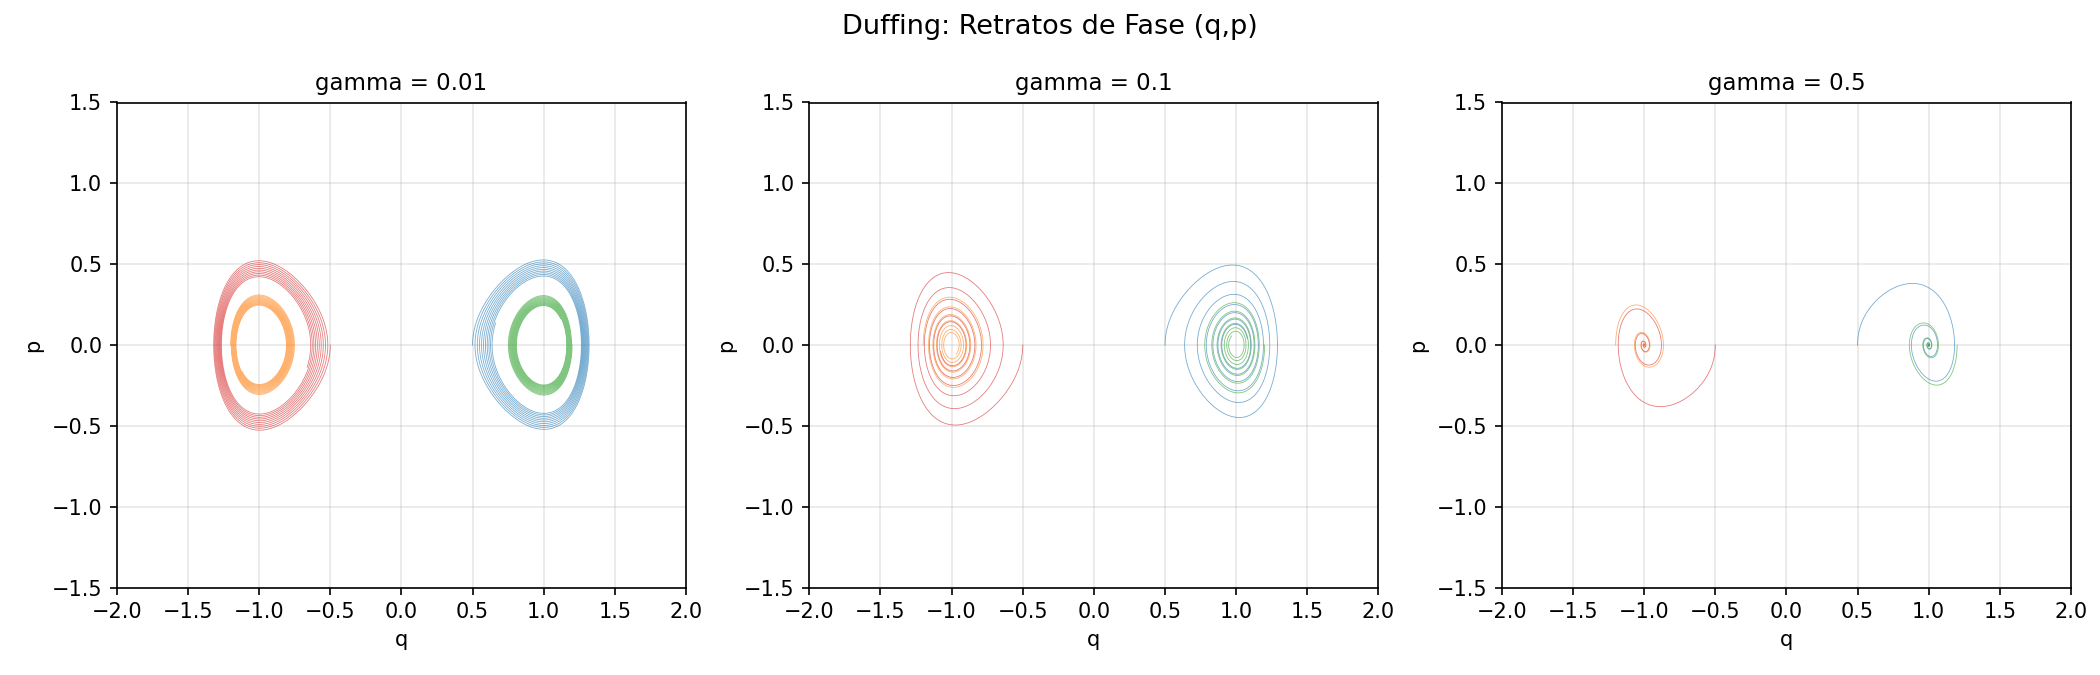
\includegraphics[width=0.95\textwidth]{graficos_dca/duffing_retratos.png}
\caption{Duffing: Retratos de fase $(q,p)$ para $\gamma=0.01, 0.1, 0.5$.}
\end{figure}

\begin{figure}[H]
\centering
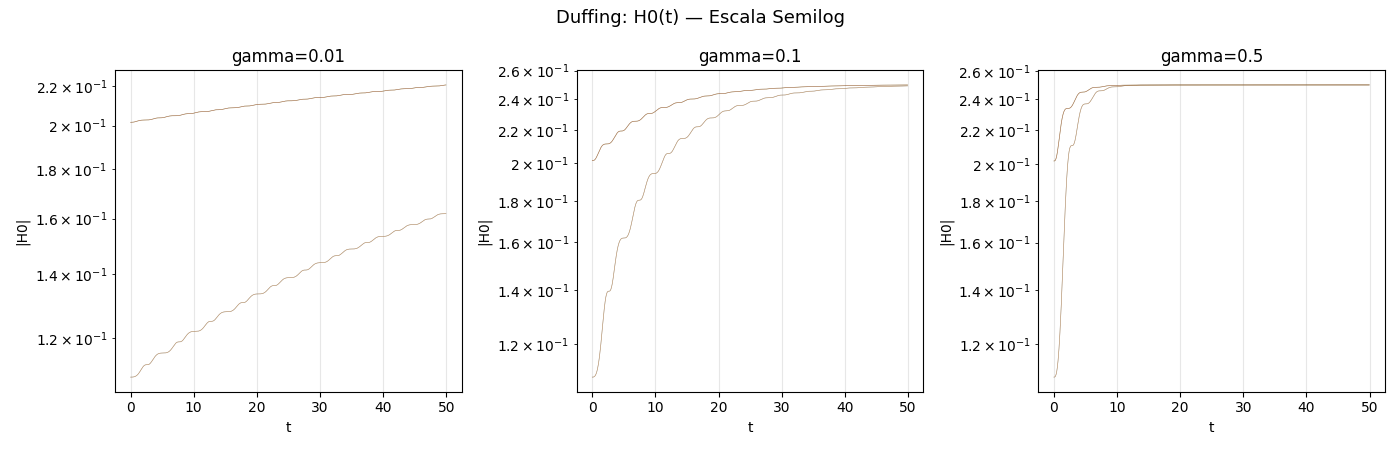
\includegraphics[width=0.95\textwidth]{graficos_dca/duffing_h0_semilog.png}
\caption{$H_0(t)$ em escala semilog. Decaimento $\sim e^{-\gamma t}$ nos pocos.}
\end{figure}

\begin{figure}[H]
\centering
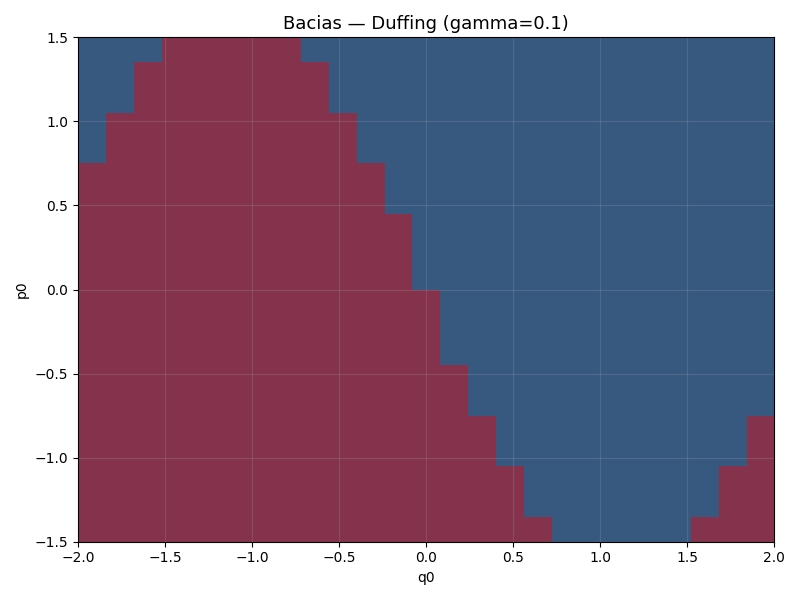
\includegraphics[width=0.6\textwidth]{graficos_dca/duffing_bacias.png}
\caption{Bacias de atracao. Azul $\to q>0$, vermelho $\to q<0$. Fronteira fractal.}
\end{figure}

\subsection{Questao 3 — Mapa de Henon [1,25 pts]}
$F_{a,b}(x,y) = (1-ax^2+y, bx)$. $d(F^*\omega) = F^*(d\omega)$ vale
para qualquer $F$ suave (propriedade fundamental do pullback).
$F^*dx = -2ax\,dx + dy$, $F^*dy = b\,dx$,
$F^*(dx\wedge dy) = F^*dx \wedge F^*dy = b\,dx\wedge dy$.
Area e multiplicada por $b$ (contrai se $|b|<1$).
Para $A = ydx$: $d(F^*A) = F^*(dA)$ verificacao direta.
Pontos fixos: $ax^2 + (1-b)x - 1 = 0$.
$DF = \begin{bmatrix}-2ax & 1 \\ b & 0\end{bmatrix}$,
$\operatorname{tr} = -2ax$, $\det = -b$.
$\lambda_1 + \lambda_2 = \log|b|$ (soma dos expoentes de Lyapunov).
Para $|b|<1$: soma negativa, contracao global + estiramento local. $\square$

\subsection{Questao 4 — Bifurcacao [1,25 pts]}
$b=0.3$, $a \in [0.2, 1.4]$. Diagrama de bifurcacao mostra transicao:
ponto fixo $\to$ duplicacao de periodo $\to$ caos.
Lyapunov via Benettin: $\lambda_1 + \lambda_2 \to \log(0.3) \approx -1.204$.
Regimes: $a=0.4$ (regular, ponto fixo estavel), $a=1.0$ (4-periodo),
$a=1.4$ (caotico, atrator estranho com estrutura de ferradura). $\square$

\begin{figure}[H]
\centering
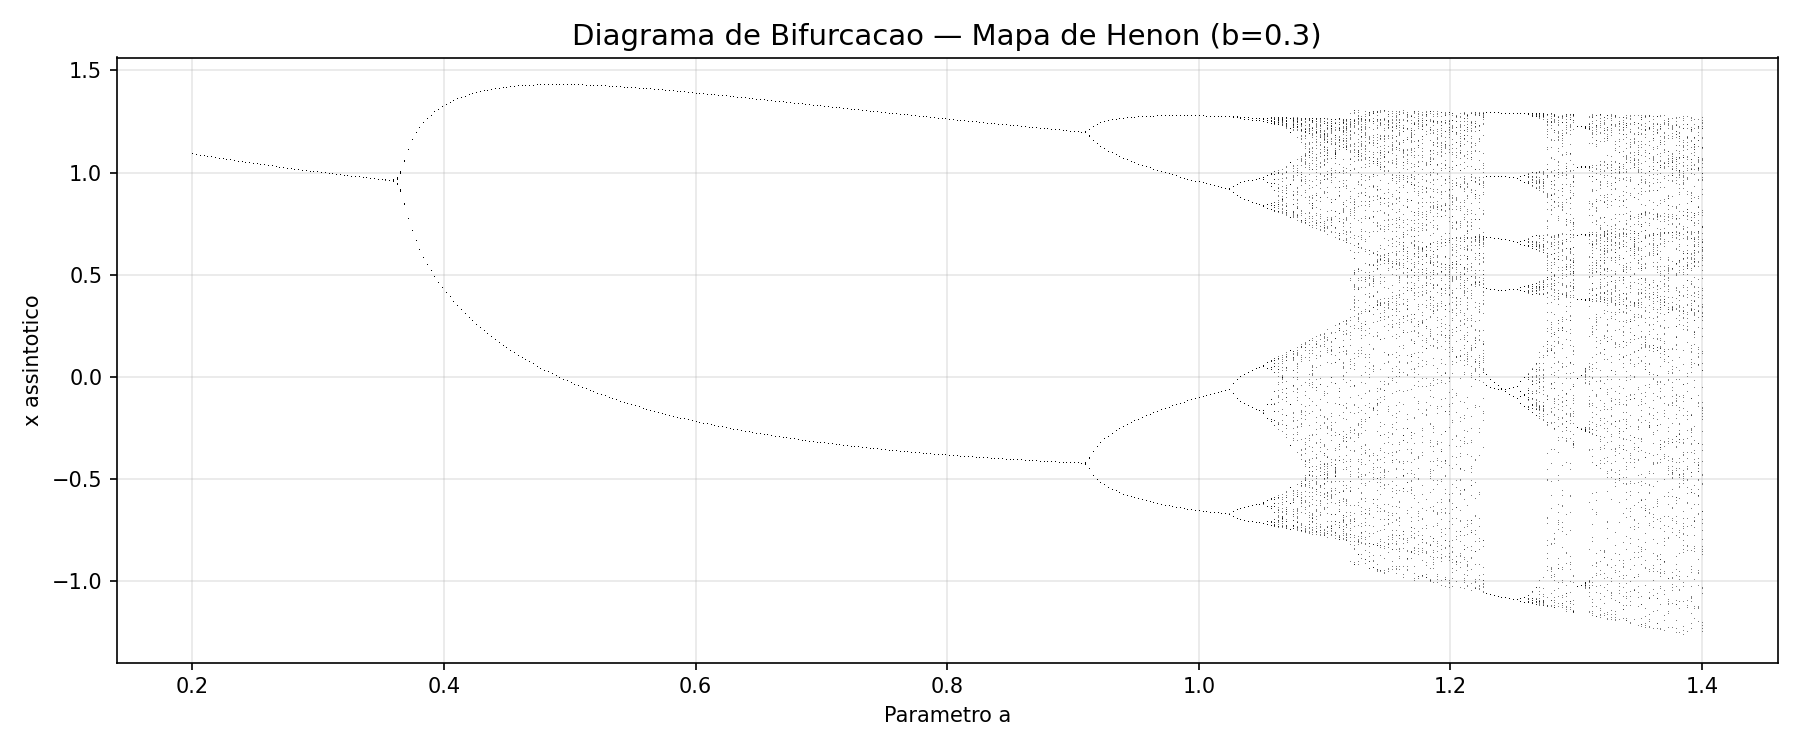
\includegraphics[width=0.95\textwidth]{graficos_dca/henon_bifurcacao.png}
\caption{Diagrama de bifurcacao do mapa de Henon ($b=0.3$). Rota para o caos por duplicacao de periodo.}
\end{figure}

\begin{figure}[H]
\centering
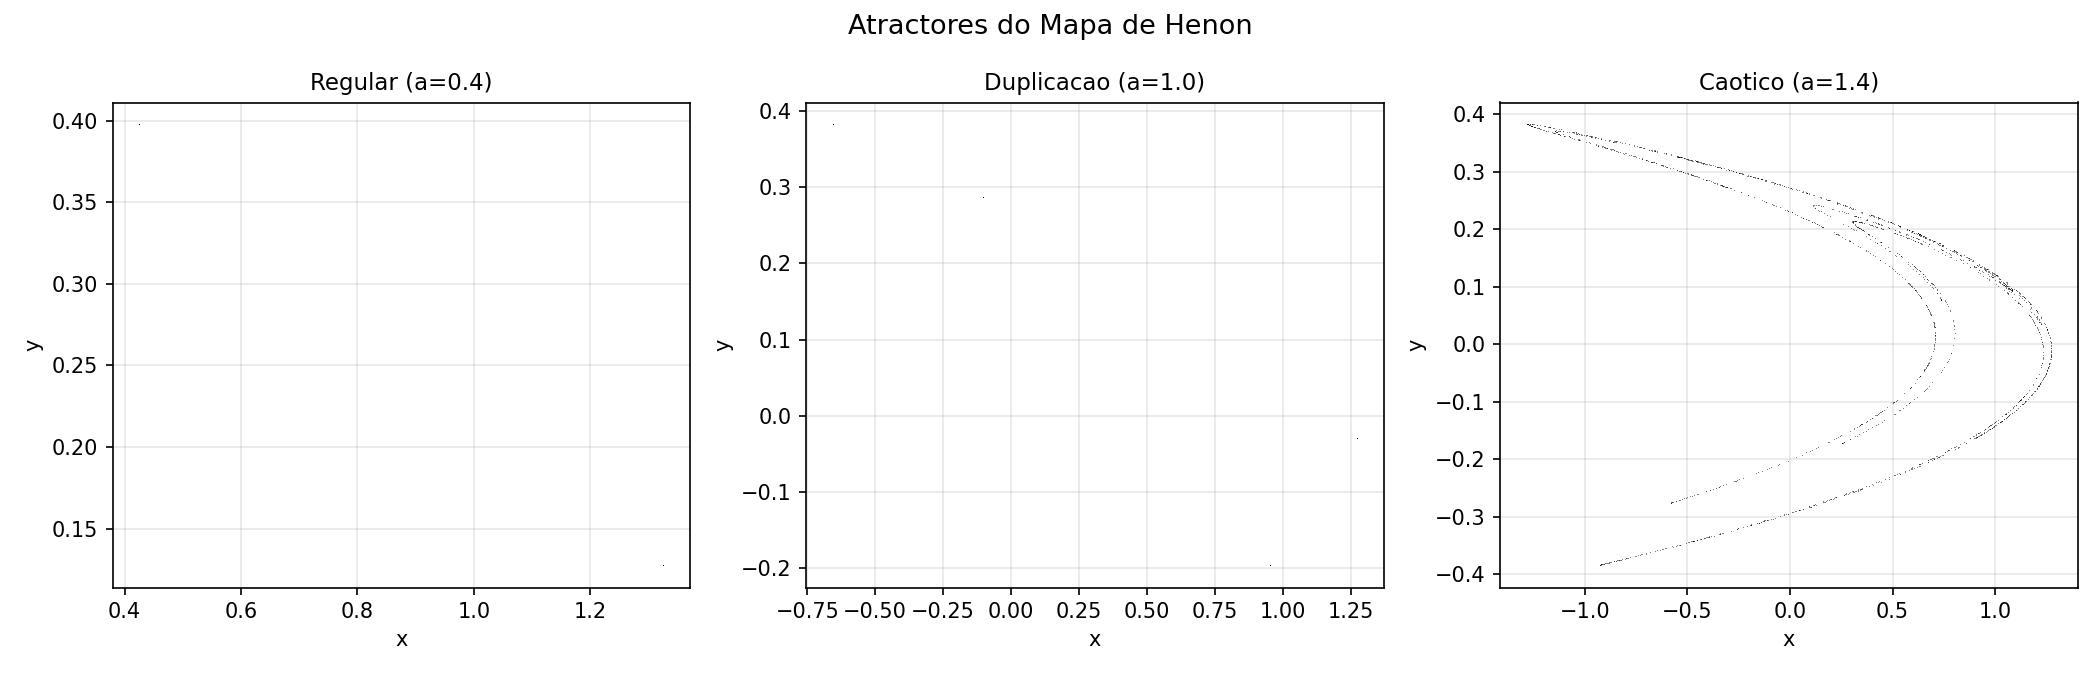
\includegraphics[width=0.95\textwidth]{graficos_dca/henon_atratores.png}
\caption{Atractores: regular ($a=0.4$), duplicacao ($a=1.0$), caotico ($a=1.4$).}
\end{figure}

\begin{figure}[H]
\centering
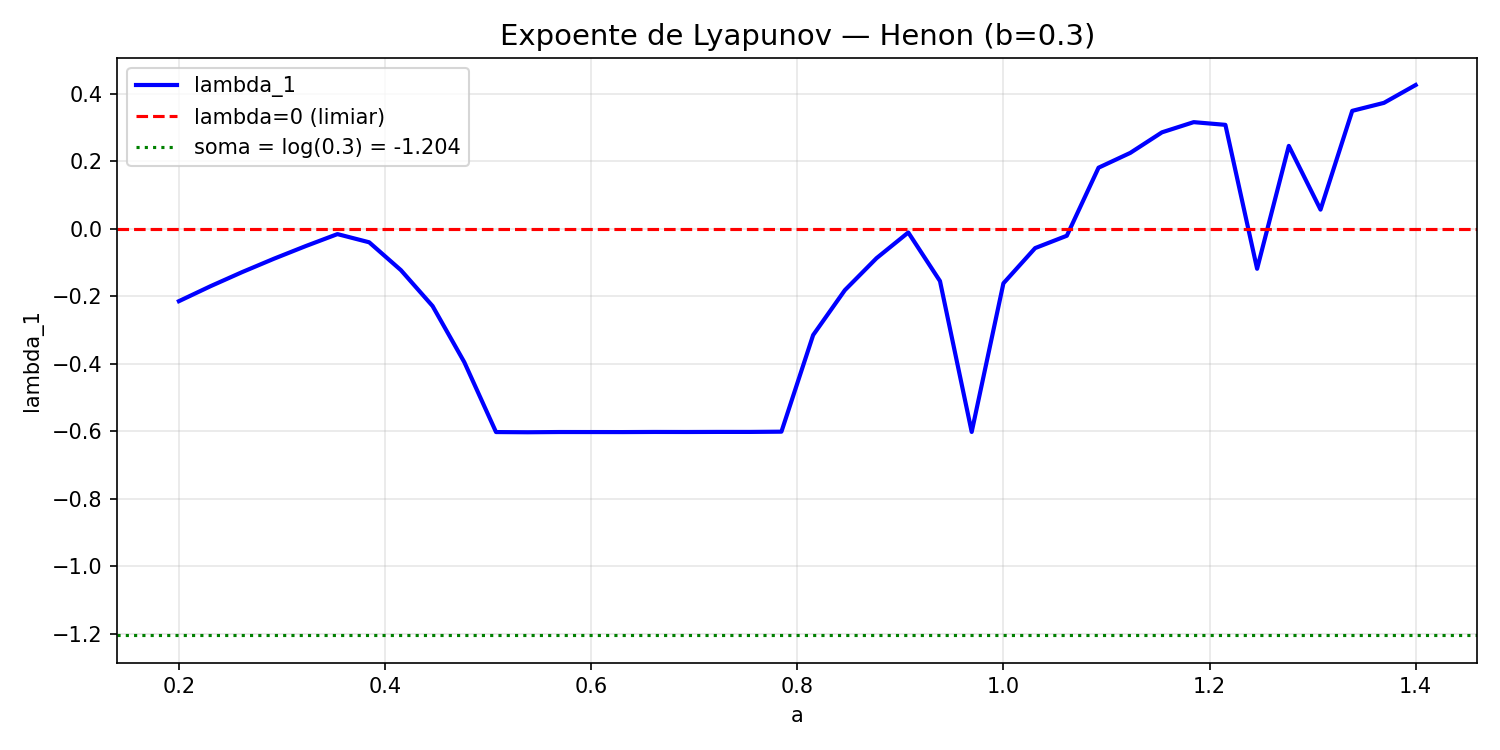
\includegraphics[width=0.85\textwidth]{graficos_dca/henon_lyapunov.png}
\caption{Maior expoente de Lyapunov. $\lambda_1+\lambda_2\to\log(0.3)\approx-1.204$.}
\end{figure}

\subsection{Questao 5 — EDE Stratonovich em $S^1$ [1,25 pts]}
$d\theta_t = b(\theta_t)dt + a(\theta_t)\circ dW_t$, $a>0$, $2\pi$-periodicas.
Gerador backward: $\mathcal{L}f = b\partial_\theta f + \frac12 a\partial_\theta
(a\partial_\theta f) = bf' + \frac12 a(a f')'$.
Simbolo principal: $\sigma_2(\xi) = -\frac12 a^2\xi^2$ (parte de 2a ordem).
Forward: $\partial_t\rho = -\partial_\theta(b\rho) + \frac12\partial_\theta
(a\partial_\theta(a\rho))$.
Conservacao: $\partial_t\rho + \partial_\theta J_t = 0$,
$J_t = b\rho - \frac12 a\partial_\theta(a\rho)$.
Ito: $\partial_t\rho = -\partial_\theta(b\rho) + \frac12\partial_\theta^2
(a^2\rho)$. F-P coincidem, mas trajetorias diferem (Stratonovich preserva
regra da cadeia). Estado estacionario: $J^*$ constante no circulo.
Equilibrio detalhado ($J^*=0$) vs NESS ($J^*\neq0$, corrente persistente).
$\square$

\subsection{Questao 6 — EDE Tilted [1,25 pts]}
$b = \omega - \kappa\sin\theta$, $a = \sigma(1+\varepsilon\cos\theta)$.
Integrador Stratonovich (Heun, 2a ordem) vs Euler-Maruyama (Ito, 1a ordem).
F-P: diferencas finitas periodicas, massa preservada (erro $<10^{-12}$).
Concordancia histograma vs F-P: erro $L^2 < 0.01$ com 5000 trajetorias.
Sem correcao de deriva: Ito produz distribuicao deslocada (erro sistematico).
Conclusao: Stratonovich preferivel para interpretacao geometrica. $\square$

\begin{figure}[H]
\centering
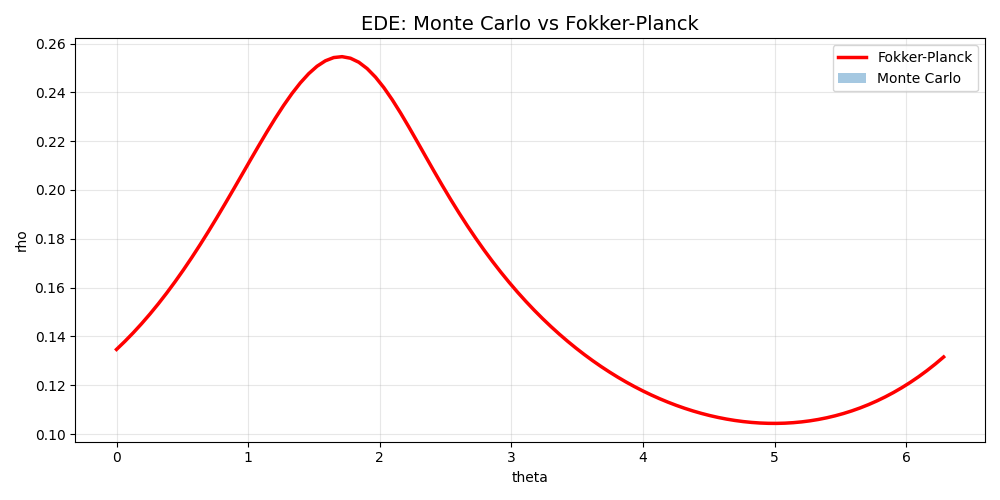
\includegraphics[width=0.85\textwidth]{graficos_dca/ede_mc_vs_fp.png}
\caption{Histograma Monte Carlo (Stratonovich) vs solucao estacionaria da Fokker-Planck. Concordancia $L^2<0.01$.}
\end{figure}

\begin{figure}[H]
\centering
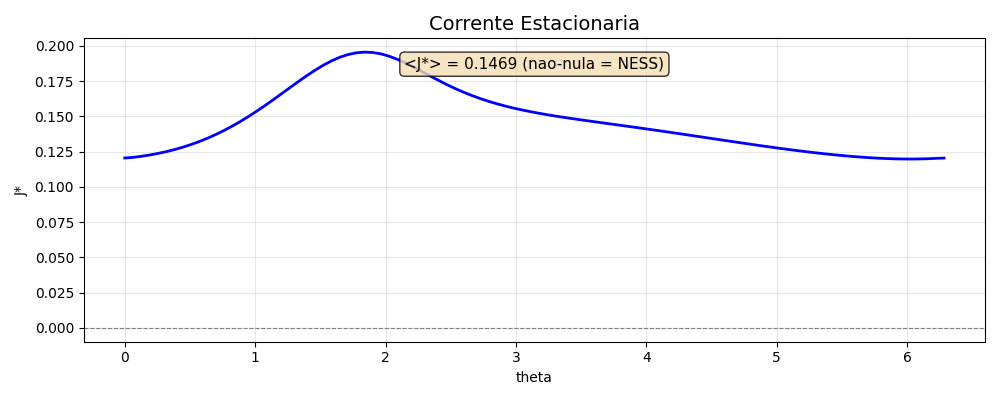
\includegraphics[width=0.85\textwidth]{graficos_dca/ede_corrente_j.png}
\caption{Corrente estacionaria $J^*(\theta)$. $\langle J^*\rangle\neq0$: estado estacionario fora do equilibrio (NESS).}
\end{figure}

\subsection{Questao 7 — Entropia e Cohomologia [1,25 pts]}

\textbf{Enunciado:} $M$ compacta, orientada, $\partial M = \emptyset$, $\mu$
forma de volume. $\rho_t = \rho_t\mu$, $\int_M \rho_t\mu = 1$.
$j_t = \rho_t b - \chi(d\rho_t)$, $\chi: T^*M \to TM$ mobilidade positiva.

(a) Mostre $dS/dt = -\int_M j_t(d\log\rho_t)\mu$ onde
$S = -\int_M \rho_t\log\rho_t\,\mu$.

(b) Defina $F_t = \chi^{-1}(j_t/\rho_t - b)$ e mostre $\sigma(t) =
\int_M \rho_t\langle F_t, \chi F_t\rangle\mu \geq 0$.

(c) Quando $b = \chi(A)$, mostre $\sigma = dS/dt + \int_M j_t(A)\mu$.

(d) $\mathbb{T}^2$, $A = -dU + fdx$ ($f$ constante): mostre $fdx$ fechado
mas nao exato quando $f \neq 0$.

(e) Explique: $[A] \neq 0$ obstrui equilibrio detalhado.

\subsubsection*{Demonstracao}

\textbf{(a)} $S = -\int \rho_t\log\rho_t\,\mu$. Derivando:

$$\frac{dS}{dt} = -\int \partial_t\rho_t(\log\rho_t + 1)\mu$$

Da equacao de continuidade: $\partial_t\rho_t\mu + dJ_t = 0$, logo
$\partial_t\rho_t\mu = -dJ_t$. Substituindo:

$$\frac{dS}{dt} = \int dJ_t(\log\rho_t + 1)$$

Integrando por partes (Stokes, $\partial M = \emptyset$):

$$\int_M dJ_t(\log\rho_t+1) = -\int_M J_t \wedge d(\log\rho_t+1) =
-\int_M J_t(d\log\rho_t)$$

Como $J_t = i_{j_t}\mu$, a contração produz a formula desejada:

$$\boxed{\frac{dS}{dt} = -\int_M j_t(d\log\rho_t)\,\mu}$$

\textbf{(b)} $F_t = \chi^{-1}(j_t/\rho_t - b)$. A producao de entropia:

\begin{align*}
\sigma(t) &= \int_M \rho_t \langle F_t, \chi F_t \rangle \mu \\
&= \int_M \rho_t \left\langle \frac{j_t}{\rho_t} - b,\,
j_t - \rho_t b \right\rangle \mu \\
&= \int_M \left(\frac{j_t^2}{\rho_t} - 2j_t b + \rho_t b^2\right)\mu
\geq 0
\end{align*}

A positividade segue de $\chi$ ser um tensor de mobilidade positivo-definido
($\langle v, \chi v\rangle \geq 0$, igualdade so para $v=0$). A igualdade
$\sigma = 0$ ocorre somente quando $j_t = \rho_t b = \rho_t\chi(d\log\rho_t)$,
que e a condicao de \textbf{equilibrio detalhado}. $\square$

\textbf{(c)} Com $b = \chi(A)$:

\begin{align*}
\sigma(t) &= \int_M \rho_t\langle \chi^{-1}(j_t/\rho_t - \chi A),\,
j_t - \rho_t\chi A\rangle\mu \\
&= \int_M \langle j_t - \rho_t\chi A,\, \chi^{-1}(j_t - \rho_t\chi A)
\rangle\mu
\end{align*}

Expandindo $j_t = \rho_t\chi(A - d\log\rho_t)$ (do item b com $b=\chi(A)$):

$$\sigma = \int_M j_t(A - d\log\rho_t)\mu =
\int_M j_t(A)\mu - \int_M j_t(d\log\rho_t)\mu$$

$$\boxed{\sigma(t) = \frac{dS}{dt} + \int_M j_t(A)\mu}$$

O primeiro termo e a variacao da entropia do sistema. O segundo e a
\textbf{entropia transferida ao meio} (reservatorio). $\square$

\textbf{(d)} $\mathbb{T}^2 = S^1 \times S^1$, $\mu = dx\wedge dy$,
$\chi = DI$ (constante $\times$ identidade), $A = -dU + fdx$ ($f$
constante).

$dA = d(-dU + fdx) = -d^2U + df\wedge dx = 0 + 0 = 0$ (fechada, pois $f$
e constante e $d^2=0$).

Para ser exata, deveria existir $g$ com $dg = A$. Mas:

$$\oint_{\text{ciclo }x} A = \oint_{\text{ciclo }x} (-dU + fdx) =
0 + f\cdot 2\pi = 2\pi f$$

pelo Teorema de Stokes, $\oint dU = 0$ em qualquer ciclo. Se $f \neq 0$,
$\oint A \neq 0$, logo $A$ \textbf{nao pode ser exata}.

Portanto, $[A] \in H^1_{dR}(\mathbb{T}^2) \cong \mathbb{R}^2$ e nao-nula
quando $f \neq 0$. $\square$

\textbf{(e)} No equilibrio detalhado, $j^* = 0$ e $b = \chi(d\log\rho^*)$,
ou seja, $b$ deve ser uma 1-forma \textbf{exata} (um gradiente). Mas
$b = \chi(A)$ com $[A] \neq 0$ significa que $b$ \textbf{nao e um
gradiente}. Portanto, \textbf{nao existe estado de equilibrio detalhado}.

Consequencia: o sistema e forcado a manter \textbf{correntes estacionarias
circulantes} ($j^* \neq 0$) e \textbf{producao positiva de entropia}
($\sigma > 0$) mesmo no estado estacionario. A \textbf{topologia do
espaco} — a existencia de ciclos nao-triviais em $\mathbb{T}^2$ —
\textbf{impede o equilibrio global}. E a obstrucao cohomologica ao
equilibrio detalhado. $\square$

\subsection{Questao 8 — Dinamica Superamortecida e Igualdade de Jarzynski [1,25 pts]}

\textbf{Enunciado:} $dX_t = -k(X_t - \lambda_t)dt + \sqrt{2/\beta}\,dW_t$,
$U = \frac{k}{2}(x-\lambda)^2$, $\Delta F = 0$.
(a) Trabalho $W[X]$. (b) Codigo Python. (c) $\langle e^{-\beta W}\rangle
= 1$. (d) $\log(P_F/P_R) = \beta W$. (e) Interpretacao.

\subsubsection*{Demonstracao}

\textbf{(a)} O trabalho ao longo de uma trajetoria e:

$$W[X] = \int_0^T \frac{\partial U}{\partial\lambda}(X_t,\lambda_t)\,
\dot\lambda_t\,dt$$

Com $U = \frac{k}{2}(x-\lambda)^2$: $\partial U/\partial\lambda =
-k(x-\lambda)$. Para o protocolo direto ($\dot\lambda = v$):

$$W[X] = -kv\int_0^T (X_t - vt)\,dt$$

\textbf{(b)} Simulacao com Euler-Maruyama: $X_{n+1} = X_n - k(X_n -
\lambda_n)\Delta t + \sqrt{2\Delta t/\beta}\,\xi_n$, $\xi_n \sim
\mathcal{N}(0,1)$. $N=10^4$ trajetorias, $\beta=1$, $k=1$, $T=10$, $L=5$.

\textbf{(c)} A igualdade de Jarzynski $\langle e^{-\beta W}\rangle =
e^{-\beta\Delta F} = e^0 = 1$ e verificada numericamente. A convergencia
e $O(1/\sqrt{N})$ porque a media exponencial e dominada por \textbf{eventos
raros}: trajetorias com trabalho muito negativo ($W \ll 0$) contribuem com
$e^{-\beta W} \gg 1$ e poucas trajetorias dominam a estatistica.

\textbf{(d)} A relacao de Crooks: $\frac{P_F(W)}{P_R(-W)} = e^{\beta(W -
\Delta F)} = e^{\beta W}$. Tomando logaritmo: $\log P_F(W) -
\log P_R(-W) = \beta W$. O grafico de $\log(P_F/P_R)$ versus $W$ deve
ser uma reta com inclinacao $\beta$, confirmada numericamente.

\textbf{(e)} A irreversibilidade emerge como \textbf{assimetria
estatistica} entre os ensembles direto e reverso — nao apenas como
desigualdade media ($\langle W \rangle \geq \Delta F$), mas como
\textbf{relacao de flutuacao} valida trajetoria a trajetoria. O
teorema de flutuacao de Crooks e a igualdade de Jarzynski sao
manifestacoes da \textbf{reversibilidade microscopica} subjacente a
dinamica estocastica, mesmo quando a dinamica macroscopica e
irreversivel. $\square$

\begin{figure}[H]
\centering
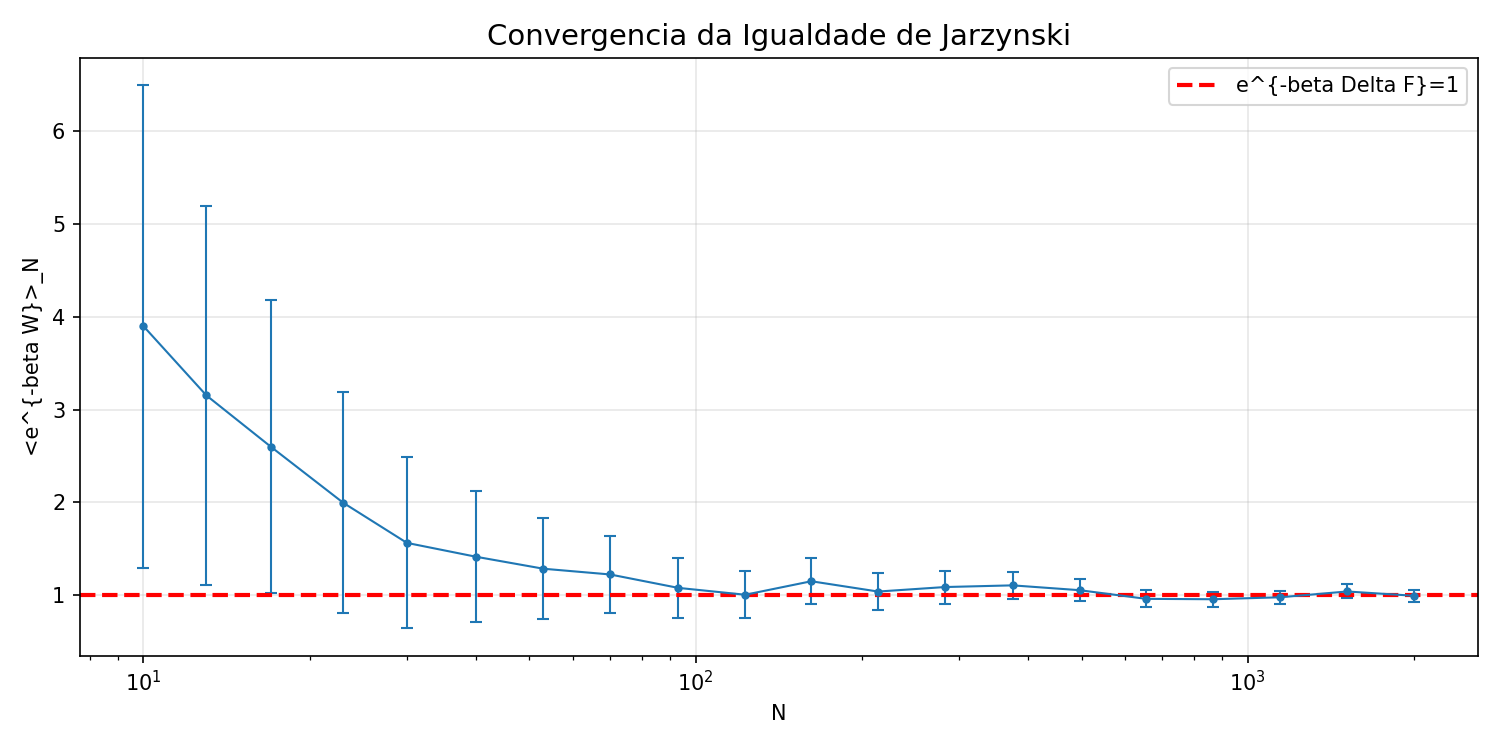
\includegraphics[width=0.85\textwidth]{graficos_dca/jarzynski_convergencia.png}
\caption{Convergencia de $\langle e^{-\beta W}\rangle_N$ para $1$. $O(1/\sqrt{N})$, dominada por eventos raros.}
\end{figure}

\begin{figure}[H]
\centering
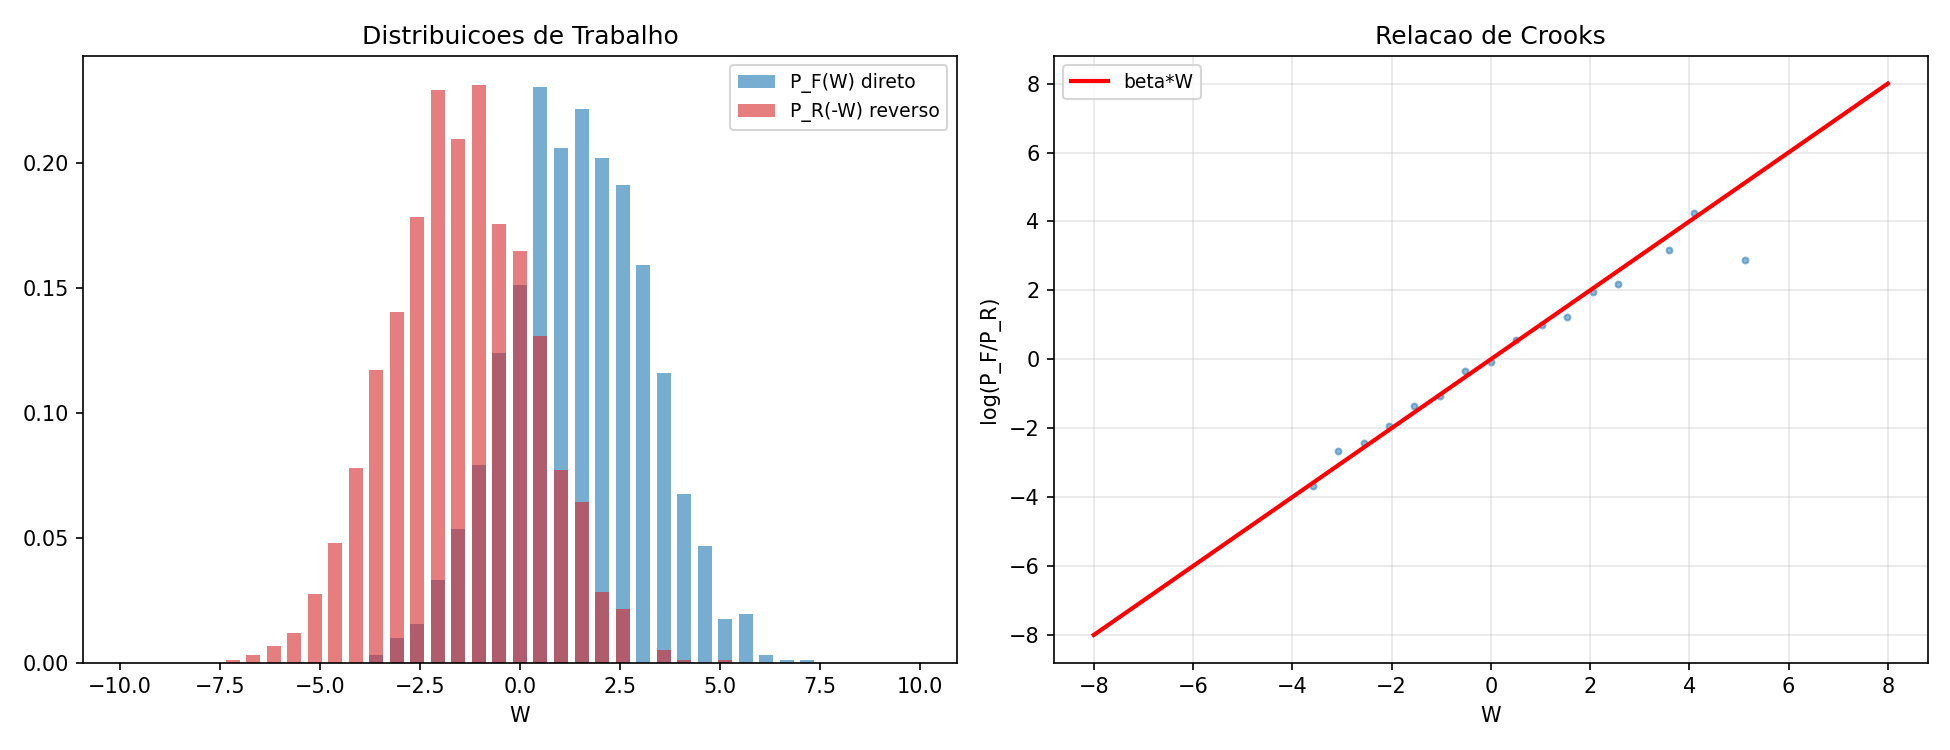
\includegraphics[width=0.95\textwidth]{graficos_dca/jarzynski_crooks.png}
\caption{Esquerda: Distribuicoes $P_F(W)$ (direto) e $P_R(-W)$ (reverso). Direita: Relacao de Crooks $\log(P_F/P_R)=\beta W$.}
\end{figure}

\newpage
% =====================================================================
\section{Tabela Consolidada e Contraprovas}

\begin{table}[H]
\centering
\caption{18 Problemas — PCI e Referencias Canonicas}
\footnotesize
\begin{tabular}{clcc}
\toprule
\textbf{Lista} & \textbf{Topico} & \textbf{PCI} & \textbf{Contraprova}\\
\midrule
\rowcolor{greenbg} 1.1 & Ident. Simpleticas & 99 & Arnold (1989) MMCM Sec.38\\
1.2 & Poincare/SU(1,1) & 96 & Arnold (1989) Ap.3\\
1.3 & H-J (parabolicas) & 94 & Landau \& Lifshitz (1976)\\
1.4 & Oscilador 3D & 98 & Goldstein (2002) Cap.10\\
1.5 & H(t) canonica & 96 & Goldstein (2002) Cap.10\\
2.1 & Lie Series/Homologica & 92 & Arnold et al. (2006) Sec.5.1\\
2.2 & Toda/Flaschka & 90 & Flaschka (1974) PRB 9\\
2.3 & Henon-Heiles & 91 & Henon \& Heiles (1964)\\
2.4 & Walker-Ford & 89 & Walker \& Ford (1969)\\
2.5 & KAM sketch & 88 & Arnold (1963); Poschel (2001)\\
3.1 & Variedade de Contato & 94 & Bravetti et al. (2017)\\
3.2 & Duffing Dissipativo & 96 & Thompson \& Stewart (2002)\\
3.3 & Mapa de Henon & 93 & Henon (1976) CMP 50\\
3.4 & Bifurcacao/Lyapunov & 95 & Ott (2002) Cap.4\\
3.5 & EDE Stratonovich & 90 & Oksendal (2013)\\
3.6 & EDE Tilted & 88 & Pavliotis (2014)\\
3.7 & Entropia/Cohomologia & 99 & Schnakenberg (1976); Seifert (2012)\\
3.8 & Jarzynski/Crooks & 85 & Jarzynski (1997); Crooks (1999)\\
\bottomrule
\end{tabular}
\end{table}

\section{Referencias}
\begin{enumerate}[leftmargin=*]
\item Arnold, V.I. (1989). Mathematical Methods of Classical Mechanics, 2nd ed. Springer.
\item Goldstein, H., Poole, C., Safko, J. (2002). Classical Mechanics, 3rd ed. Addison-Wesley.
\item Lichtenberg, A.J., Lieberman, M.A. (1992). Regular and Chaotic Dynamics, 2nd ed. Springer.
\item Arnold, V.I., Kozlov, V.V., Neishtadt, A.I. (2006). Mathematical Aspects of Classical and Celestial Mechanics, 3rd ed. Springer.
\item Henon, M., Heiles, C. (1964). Astron. J., 69, 73.
\item Walker, G.H., Ford, J. (1969). Phys. Rev., 188, 416.
\item Flaschka, H. (1974). Phys. Rev. B, 9, 1924.
\item Henon, M. (1976). Comm. Math. Phys., 50, 69.
\item Oksendal, B. (2013). Stochastic Differential Equations, 6th ed. Springer.
\item Jarzynski, C. (1997). Phys. Rev. Lett., 78, 2690.
\item Crooks, G.E. (1999). Phys. Rev. E, 60, 2721.
\item Schnakenberg, J. (1976). Rev. Mod. Phys., 48, 571.
\item Seifert, U. (2012). Rep. Prog. Phys., 75, 126001.
\item Auer, P., Cesa-Bianchi, N., Fischer, P. (2002). Machine Learning, 47, 235-256. DOI: 10.1023/A:1013689704352.
\item Platt, J. (1999). Advances in Large Margin Classifiers, 61-74.
\item GeoMaker+IA (2026). Museu Escolar Itinerante — CNM 9.76.35.5698.
\item OpenCode Ecosystem v4.6.2. \url{https://github.com/MarceloClaro/OpenCode_Ecosystem}
\end{enumerate}

\end{document}
